\setlength{\baselineskip}{20pt}
\chapter{基于模型蒸馏的特征增强算法研究}
\label{cha:chap4}

第三章提出的面向无额外推理成本的特征增强算法，通过参数融合机制实现了去噪操作的零额外推理开销。然而，该方法存在两个固有的局限性：其一，去噪模块必须被设计为与嵌入层参数可融合的轻量化结构，有限的参数规模制约了其对复杂噪声分布的建模能力，导致去噪精度存在提升空间；其二，去噪步数受限于骨干网络的层数，当网络深度有限时，可用的去噪幅度相应受限。针对上述两个问题，本章提出基于模型蒸馏的特征增强算法，引入两项协同增强策略加以解决。第\ref{sec:chap4_evolution}节分析从参数融合到蒸馏增强的问题演进；第\ref{sec:chap4_distill}节提出教师--学生蒸馏去噪框架以增强轻量级去噪模块的建模能力；第\ref{sec:chap4_multi}节设计有限去噪深度下的增强策略，包括多轮单层去噪和多步去噪融合；第\ref{sec:chap4_paradigm}节讨论无监督与有监督学习范式的统一；第\ref{sec:chap4_exp_setup}节和第\ref{sec:chap4_exp_result}节分别介绍实验设置与结果分析；最后在第\ref{sec:chap4_summary}节对本章工作进行总结。

\section{从参数融合到蒸馏增强的问题演进}
\label{sec:chap4_evolution}

第三章所提方法的核心优势在于通过参数融合实现零额外推理开销，但这一设计在带来高效性的同时，也对去噪模块的结构施加了严格约束。具体而言，为了保证去噪层参数$W_D$能够与嵌入层参数$W$进行等价融合（式（\ref{eq:chap3_w_prime}）），去噪模块必须是一个与嵌入层维度匹配的线性变换。这意味着去噪模块的参数量与原始嵌入层相当，其表达能力受到了内在限制。

从噪声建模的角度分析，轻量级去噪模块面临的核心挑战在于：实际判别式任务中的特征噪声往往具有复杂的、非各向同性的分布特征。例如，在行人重识别任务中，噪声可能来源于遮挡区域的特征坍缩、跨视角变化引起的特征漂移以及背景杂乱造成的干扰信号，这些噪声的分布具有高度的空间相关性和任务依赖性。有限参数规模的去噪模块难以精确捕获这些复杂的噪声模式，导致噪声预测存在系统性偏差。

另一方面，第三章方法中每一层执行一步去噪（$Y_t \rightarrow Y_{t-1}$），整个骨干网络的$N$个嵌入层完成$N$步去噪（$Y_N \rightarrow Y_0$）。对于层数较少的骨干网络（如12层的ViT-small），可用的去噪步数仅为12步，这在面对高噪声场景时可能不足以将特征充分去噪至干净分布。虽然第三章已经推导了两步去噪的扩展公式（式（\ref{eq:chap3_two_step_combined}）），但简单地增加每层的去噪步数会引入离散化误差的累积问题，需要更加精细的策略来保证去噪质量。

基于上述分析，本章提出两项互补的增强策略：

（1）教师--学生蒸馏增强。利用一个表达能力更强的教师网络在训练阶段指导轻量级学生去噪模块的学习。教师网络能够更准确地捕获噪声的结构化模式，通过蒸馏将这种能力传递给学生模块，有效校正学生的噪声预测偏差，从而在不改变推理结构的前提下提升去噪精度。

（2）多步去噪融合。通过多轮单层去噪和逐步蒸馏，将多步去噪轨迹压缩为等效的单步操作。这一策略在有限的网络层数下模拟更深的去噪轨迹，增强去噪幅度，同时保持参数融合的零额外推理开销特性。

这两项策略从不同维度解决第三章方法的局限性：蒸馏增强提升去噪的精度，多步融合扩大去噪的幅度。两者协同作用，使得增强后的方法能够在保持零推理开销的前提下获得更强的特征去噪能力。

\section{教师--学生蒸馏去噪框架}
\label{sec:chap4_distill}

本节提出教师--学生蒸馏去噪框架，通过利用高容量教师网络的知识指导轻量级学生去噪模块的训练，在不改变推理阶段网络结构的前提下，显著提升去噪模块的噪声预测精度。

\subsection{问题分析}

如第\ref{sec:chap4_evolution}节所述，第三章方法中的去噪模块$D_\theta$被设计为与嵌入层维度匹配的线性变换，以满足参数融合的需求。然而，线性变换的表达能力受限于其参数空间的维度，面对高维特征空间中复杂的噪声分布时，其噪声预测$\hat{\boldsymbol{\epsilon}}_S(\mathbf{x}_t, t)$与真实噪声$\boldsymbol{\epsilon}$之间存在不可忽视的系统性偏差。

具体而言，这种偏差的来源可以从两个方面理解。首先，从函数逼近的角度，线性去噪模块只能学习噪声分布的一阶近似，而实际噪声分布中的高阶相关性（如不同通道之间的噪声耦合）无法被精确建模。其次，从优化的角度，当去噪损失$\mathcal{L}_p = \sum_{i=1}^{N}\|\boldsymbol{\epsilon}_i - D_{\theta_i}(\mathbf{x}_{t_i}, t_i)\|^2$收敛后，残余误差反映的是模型容量的上限而非训练不充分。

为了突破这一能力瓶颈，本章借鉴知识蒸馏\cite{hinton2015distilling}的思想：在训练阶段引入一个参数量更大、表达能力更强的教师网络$D_T$，通过教师对噪声分布的更精确建模来指导学生网络$D_S$的学习。关键在于，教师网络仅在训练阶段使用，推理阶段仍然只使用轻量级学生网络并通过参数融合消除额外开销，从而保持零额外推理成本的核心特性。

\subsection{蒸馏框架设计}

\begin{figure}[htbp]
    \centering
    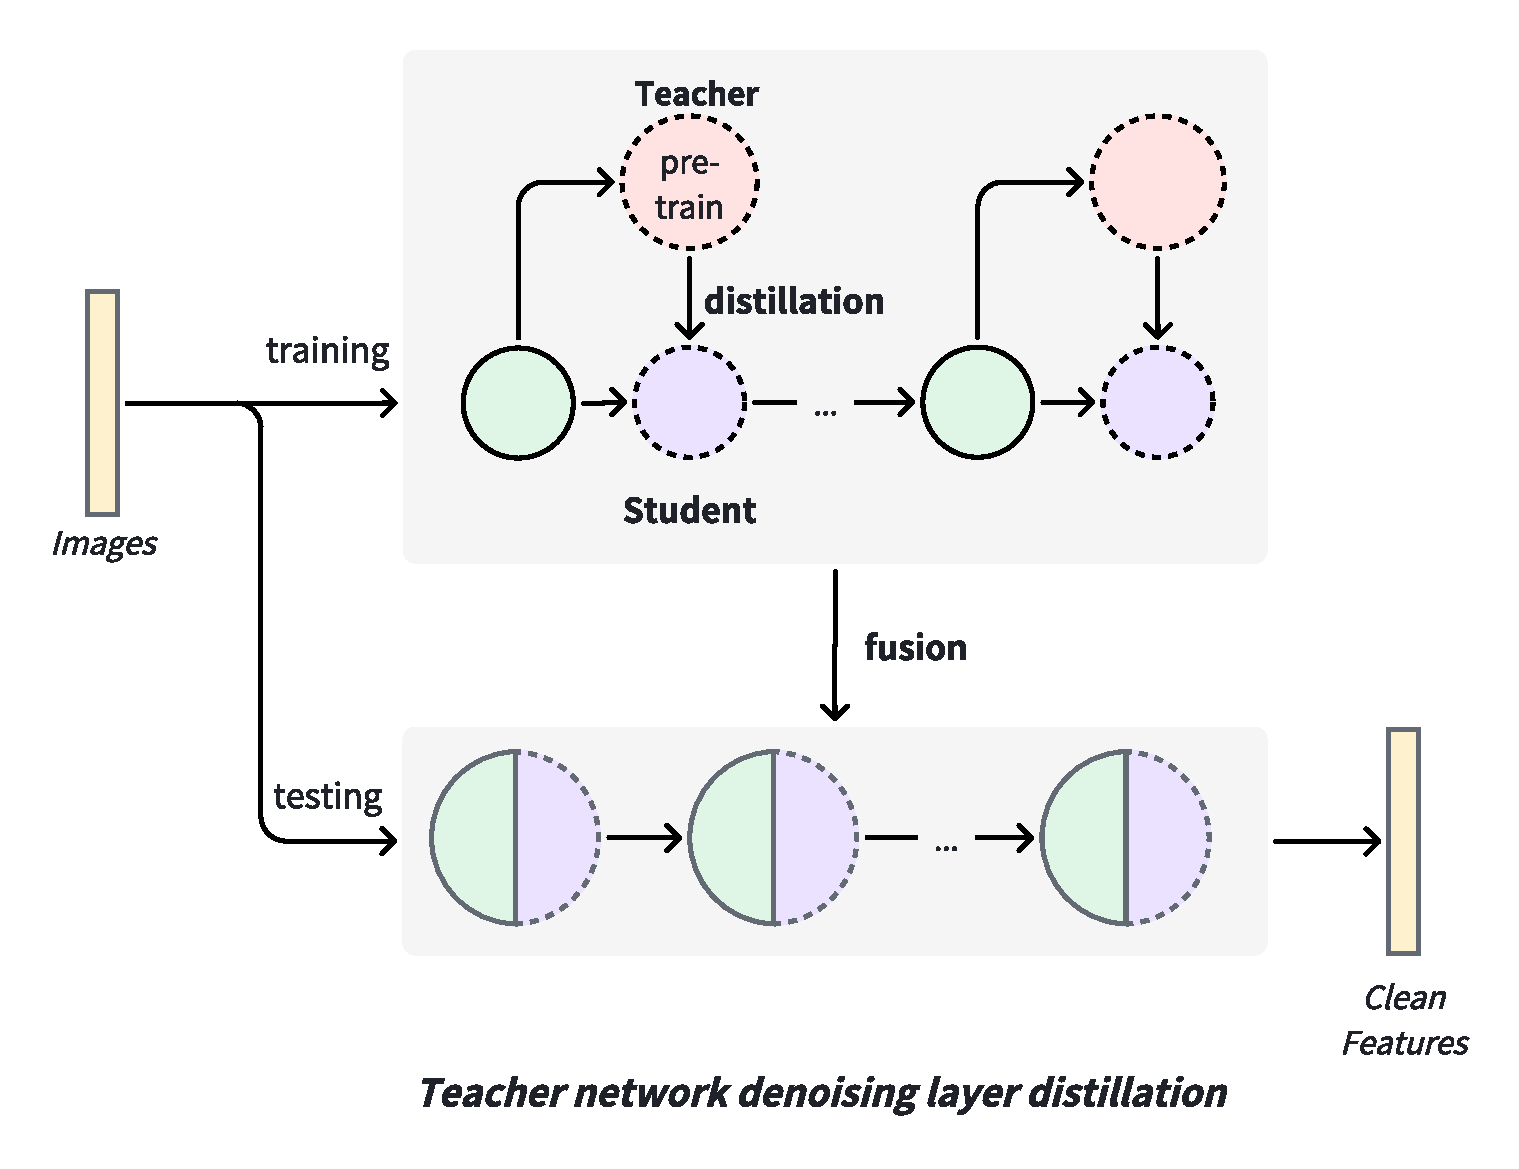
\includegraphics[width=0.95\textwidth]{figures/denoising_layer_distillation.pdf}
    \caption{教师--学生蒸馏去噪框架示意图\protect\\[-2pt]{\rm Fig.\;\thefigure\quad Illustration of the teacher--student denoising layer distillation framework}}\label{fig:chap4_distill}
\end{figure}

如图\ref{fig:chap4_distill}所示，本方法的蒸馏框架包含三个阶段：教师训练、知识蒸馏和参数融合推理。

在教师训练阶段，构建一个高容量的教师去噪网络$D_T$。与学生网络$D_S$相比，教师网络采用更宽或更深的网络结构，从而拥有更强的噪声分布建模能力。对于骨干网络第$i$层的含噪特征$\mathbf{x}_{t_i}$，教师网络输出的噪声预测为$\hat{\boldsymbol{\epsilon}}_T(\mathbf{x}_{t_i}, t_i)$，其训练目标与第三章相同：
\begin{equation}
\mathcal{L}_{teacher} = \sum_{i=1}^{N}\left\|\boldsymbol{\epsilon}_i - \hat{\boldsymbol{\epsilon}}_T(\mathbf{x}_{t_i},\, t_i)\right\|^2
\label{eq:chap4_teacher_loss}
\end{equation}
由于教师网络不受参数融合约束，其参数量可以根据实际需求灵活设定，因此能够学习到更加精确的噪声分布估计。

在知识蒸馏阶段，利用已训练好的教师网络作为软标签来指导学生网络的训练。具体而言，对于相同的含噪输入$\mathbf{x}_{t_i}$，教师网络的噪声预测$\hat{\boldsymbol{\epsilon}}_T(\mathbf{x}_{t_i}, t_i)$作为蒸馏目标，学生网络通过最小化与教师预测之间的差异来学习：
\begin{equation}
\mathcal{L}_{distill} = \sum_{i=1}^{N}\left\|\hat{\boldsymbol{\epsilon}}_S(\mathbf{x}_{t_i},\, t_i) - \hat{\boldsymbol{\epsilon}}_T(\mathbf{x}_{t_i},\, t_i)\right\|_2^2
\label{eq:chap4_distill_loss}
\end{equation}
其中$\hat{\boldsymbol{\epsilon}}_S$和$\hat{\boldsymbol{\epsilon}}_T$分别为学生和教师网络的噪声预测。

将蒸馏损失与原始去噪损失进行加权组合，得到学生网络的整体训练目标：
\begin{equation}
\mathcal{L}_{total} = \lambda_p\,\mathcal{L}_{denoise} + \lambda_d\,\mathcal{L}_{distill}
\label{eq:chap4_total_distill}
\end{equation}
其中$\lambda_p$和$\lambda_d$为平衡两个损失项的权重系数，$\mathcal{L}_{denoise}$为第三章定义的去噪损失（式（\ref{eq:chap3_denoise_loss}））。通过联合优化，学生网络既能从真实噪声标签中学习基本的去噪能力，又能从教师的预测中获取更精细的噪声结构信息。

教师--学生蒸馏训练的完整算法如算法\ref{alg:chap4_distill}所示。

\begin{algorithm}[htbp]
\caption{教师--学生蒸馏训练算法}
\label{alg:chap4_distill}
\begin{algorithmic}[1]
\REQUIRE 各层特征$\{F_i\}_{i=1}^{N}$，学生去噪模块$\{D^S_i(\cdot)\}_{i=1}^{N}$，教师去噪模块$\{D^T_i(\cdot)\}_{i=1}^{N}$，权重系数$\lambda_p$和$\lambda_d$。
\REPEAT
\FOR {每一层 $i \in [N, 1]$}
\STATE $t = i$；采样噪声 $\boldsymbol{\epsilon} \sim \mathcal{N}(\mathbf{0}, \mathbf{I})$。
\STATE $\mathbf{x}_t = \sqrt{\bar{a}_t}\,F_i + \sqrt{1-\bar{a}_t}\,\boldsymbol{\epsilon}$：执行前向扩散。
\STATE 教师预测：$\hat{\boldsymbol{\epsilon}}_T = D^T_i(\mathbf{x}_t, t)$。
\STATE 学生预测：$\hat{\boldsymbol{\epsilon}}_S = D^S_i(\mathbf{x}_t, t)$。
\STATE 计算损失 $\mathcal{L} = \lambda_p\|\boldsymbol{\epsilon} - \hat{\boldsymbol{\epsilon}}_S\|^2 + \lambda_d\|\hat{\boldsymbol{\epsilon}}_S - \hat{\boldsymbol{\epsilon}}_T\|^2$。
\STATE 对学生参数执行梯度下降步。
\ENDFOR
\UNTIL{收敛}
\end{algorithmic}
\end{algorithm}

通过蒸馏训练，学生去噪模块能够继承教师网络对噪声分布的更精确估计。在推理阶段，仅使用训练好的学生网络参数，按照第三章的参数融合方法（式（\ref{eq:chap3_w_prime}）--（\ref{eq:chap3_b_prime}））将其合并至骨干网络的嵌入层中，不引入任何额外的推理开销。这种"训练时增强、推理时融合"的设计理念，使得蒸馏带来的性能提升能够在保持零推理成本的前提下得到保留。

\section{有限去噪深度下的增强策略}
\label{sec:chap4_multi}

第\ref{sec:chap4_distill}节通过蒸馏提升了去噪模块的预测精度，但并未解决去噪幅度受限于网络层数的问题。本节提出两种互补的增强策略：多轮单层去噪通过在单层上反复执行去噪来模拟更深的去噪轨迹；多步去噪融合通过逐步蒸馏将多步去噪压缩为等效的单步操作。

\subsection{多轮单层去噪}

多轮单层去噪的核心思想是：在不增加网络层数的前提下，允许单个去噪层在同一特征上迭代执行多轮去噪，从而模拟更长的去噪轨迹。

具体而言，对于骨干网络中某一层对应的去噪模块，其基本的一步去噪操作定义为：
\begin{equation}
\mathbf{x}_{t-1} = \frac{1}{\sqrt{a_t}}\!\left(\mathbf{x}_t - \frac{1-a_t}{\sqrt{1-\bar{a}_t}}\,\boldsymbol{\epsilon}_\theta(\mathbf{x}_t,\, t)\right) + \delta_t\,\mathbf{z}
\label{eq:chap4_multi_basic}
\end{equation}
其中$\boldsymbol{\epsilon}_\theta(\mathbf{x}_t, t)$为去噪模块预测的噪声，$\delta_t\,\mathbf{z}$为高斯扰动项。

假设去噪模块为线性层$G_\theta(\mathbf{x}_t, t) = W\mathbf{x}_t + b$，式（\ref{eq:chap4_multi_basic}）可改写为仿射变换形式。定义：
\begin{equation}
\left\{\;\begin{aligned}
A_t &= \sqrt{a_t}\!\left(\mathbf{I} - \frac{1-a_t}{\sqrt{1-\bar{a}_t}}\,W\right) \\[4pt]
C_t &= -\frac{1-a_t}{\sqrt{1-\bar{a}_t}}\,b
\end{aligned}\right.
\label{eq:chap4_affine_def}
\end{equation}
则一步去噪的递推关系简化为：
\begin{equation}
\mathbf{x}_{t-1} = A_t\,\mathbf{x}_t + C_t + \delta_t\,\mathbf{z}
\label{eq:chap4_recursive}
\end{equation}

将式（\ref{eq:chap4_recursive}）递推$k$步，可以得到从$\mathbf{x}_t$到$\mathbf{x}_{t-k}$的多轮去噪结果：
\begin{equation}
\begin{aligned}
\mathbf{x}_{t-k} &= \Bigl(\prod_{j=0}^{k-1}A_{t-j}\Bigr)\,\mathbf{x}_t + \sum_{j=0}^{k-1}\Bigl(\prod_{m=j+1}^{k-1}A_{t-m}\Bigr)\,C_{t-j} \\
&\quad + \sum_{j=0}^{k-1}\Bigl(\prod_{m=j+1}^{k-1}A_{t-m}\Bigr)\,\delta_{t-j}\,\mathbf{z}
\end{aligned}
\label{eq:chap4_kstep}
\end{equation}
其中$\prod_{m=j+1}^{k-1}A_{t-m}$为系数矩阵的连乘项。由于$A_t$和$C_t$均可预先计算，上述多轮去噪的结果仍然可以表示为关于$\mathbf{x}_t$的仿射变换，从而支持与嵌入层参数的融合。

将多轮去噪结果与线性嵌入层$Y = W_L\mathbf{x} + b_L$组合后，最终的特征输出为：
\begin{equation}
Y_0 = W_L\bigl(A_t\,\mathbf{x}_t + C_t + \delta_t\,\mathbf{z}\bigr) + b_L
\label{eq:chap4_multi_output}
\end{equation}
该表达式可以抽象为融合函数$Y_0 = f_{\text{fusion}}(\mathbf{x}_t, t, W_L, b_L, W, b)$，其中所有中间变量均可在推理前预计算完成。

\subsection{多步去噪融合}

多轮单层去噪虽然能够增加去噪幅度，但直接递推可能引入离散化误差的累积。为此，本节进一步引入多步去噪融合策略，借鉴渐进蒸馏\cite{salimans2022progressive}的思想，通过教师网络的多步去噪结果指导学生网络学习等效的单步去噪。

该策略的实施分为三个阶段，如算法\ref{alg:chap4_multi_step}所示。

在第一阶段（教师多步去噪），利用已训练好的教师去噪网络$D_T$，采用类似DDIM\cite{song2020denoising}的跳步采样规则，对含噪特征$\mathbf{z}_t$执行多步（$k \geq 2$步）去噪，得到去噪后的特征$\hat{\mathbf{x}}$：
\begin{equation}
\mathbf{z}_t \xrightarrow{D_T,\,k\text{步}} \hat{\mathbf{x}}
\label{eq:chap4_teacher_multistep}
\end{equation}
教师网络的基础训练目标为标准的去噪损失：
\begin{equation}
\mathcal{L}_{\theta} = \left\|\boldsymbol{\epsilon} - \hat{\boldsymbol{\epsilon}}_\theta(\mathbf{z}_t,\, t)\right\|_2^2
\label{eq:chap4_teacher_base}
\end{equation}
其中$\boldsymbol{\epsilon}$为采样的高斯噪声，$\hat{\boldsymbol{\epsilon}}_\theta$为教师的噪声预测。

在第二阶段（学生单步预测），学生网络$D_S$对相同的含噪输入$\mathbf{z}_t$执行单步预测，直接输出去噪结果$\hat{\mathbf{x}}_S$。学生网络的训练目标是逼近教师多步去噪的结果：
\begin{equation}
\mathcal{L}_{fusion} = w(\lambda_t)\left\|\hat{\mathbf{x}} - \hat{\mathbf{x}}_S(\mathbf{z}_t,\, t)\right\|_2^2
\label{eq:chap4_fusion_loss}
\end{equation}
其中$\hat{\mathbf{x}}$为教师多步去噪的输出，$\hat{\mathbf{x}}_S(\mathbf{z}_t, t)$为学生的单步预测，$w(\lambda_t)$为与时间步相关的加权函数。

在第三阶段（参数融合推理），训练完成后的学生网络参数按照第三章的融合公式合并至骨干网络嵌入层，实现零额外推理开销的多步去噪效果。

\begin{algorithm}[htbp]
\caption{多步去噪融合算法}
\label{alg:chap4_multi_step}
\begin{algorithmic}[1]
\REQUIRE 训练样本$\mathbf{x}$，扩散步数$t$，噪声调度$\{\beta_t\}$，教师去噪网络$D_T$，学生去噪网络$D_S$。
\ENSURE 融合后的学生模型，具备单步实现多步去噪的能力。
\STATE \underline{阶段一}：训练教师网络。
\FOR {每个小批量$\mathbf{x}$}
\STATE 采样噪声 $\boldsymbol{\epsilon} \sim \mathcal{N}(\mathbf{0}, \mathbf{I})$。
\STATE 前向扩散：$\mathbf{z}_t = \sqrt{\bar{a}_t}\,\mathbf{x} + \sqrt{1-\bar{a}_t}\,\boldsymbol{\epsilon}$。
\STATE 教师预测噪声 $\hat{\boldsymbol{\epsilon}}_T = D_T(\mathbf{z}_t, t)$。
\STATE 更新教师参数，最小化 $\mathcal{L}_\theta = \|\boldsymbol{\epsilon} - \hat{\boldsymbol{\epsilon}}_T\|_2^2$。
\ENDFOR
\STATE \underline{阶段二}：教师多步去噪。
\FOR {每个训练步}
\STATE 教师执行多步去噪 $\mathbf{z}_t \rightarrow \mathbf{z}_{t-k} \rightarrow \hat{\mathbf{x}}$，跳步间隔$k \geq 2$。
\ENDFOR
\STATE \underline{阶段三}：学生单步学习。
\FOR {每个小批量}
\STATE 学生单步预测 $\hat{\mathbf{x}}_S = D_S(\mathbf{z}_t, t)$。
\STATE 计算融合损失 $\mathcal{L}_{fusion} = w(\lambda_t)\|\hat{\mathbf{x}} - \hat{\mathbf{x}}_S\|_2^2$。
\STATE 更新学生参数。
\ENDFOR
\STATE 返回训练好的学生模型。
\end{algorithmic}
\end{algorithm}

这一策略的关键优势在于：教师网络通过多步迭代能够沿着更精确的去噪轨迹恢复干净特征，而学生网络通过蒸馏学习将这一多步轨迹压缩为单步操作。与直接在单层上递推多轮相比，多步去噪融合通过教师的轨迹引导有效减少了离散化误差的累积，同时保持了参数融合的可行性。实验中，模拟轮数$k$通常取较小值（$k = 2 \sim 3$），在获得显著提升的同时避免过度增加训练复杂度。

\section{无监督与有监督学习范式}
\label{sec:chap4_paradigm}

本章所提的教师--学生蒸馏增强和多步去噪融合策略，与第三章的基础方法一样，本质上均为生成式建模框架——通过学习特征的噪声分布来实现去噪，不需要任何标签信息的参与。因此，整个训练过程可以在完全无监督的条件下完成。

在无监督训练模式下，总训练损失仅包含去噪相关的损失项：
\begin{equation}
\mathcal{L}_{unsup} = \lambda_p\,\mathcal{L}_{denoise} + \lambda_d\,\mathcal{L}_{distill} + \lambda_f\,\mathcal{L}_{fusion}
\label{eq:chap4_unsup}
\end{equation}
其中$\mathcal{L}_{denoise}$为基础去噪损失（式（\ref{eq:chap3_denoise_loss}）），$\mathcal{L}_{distill}$为蒸馏损失（式（\ref{eq:chap4_distill_loss}）），$\mathcal{L}_{fusion}$为多步融合损失（式（\ref{eq:chap4_fusion_loss}）），$\lambda_p$、$\lambda_d$和$\lambda_f$为各项的平衡系数。

这意味着本方法可以利用大量无标签数据进行训练，具有良好的实用性。例如，在行人重识别任务中，可以将多个数据集的无标签图像合并进行去噪模块的训练，从而获得泛化能力更强的去噪参数。

当标签信息可用时，可以将任务特定的有监督损失$\mathcal{L}_l$引入训练框架，与去噪损失进行加权组合：
\begin{equation}
\mathcal{L}_{sup} = (1-\lambda)\,\mathcal{L}_l + \lambda\,\mathcal{L}_{unsup}
\label{eq:chap4_sup}
\end{equation}
其中$\lambda$为平衡有监督损失与去噪损失的权重系数。有监督信号能够为去噪模块提供任务层面的约束，使去噪方向更加契合下游任务的需求。第三章的实验已经初步验证了标签信息的互补性（表\ref{tab:chap3_label}），本章将在更广泛的任务和骨干网络上进一步验证这一结论。

值得指出的是，无监督与有监督范式的统一是本方法的一个重要特点。在实际应用中，许多场景下标注数据稀缺或获取成本高昂，而无标签数据则相对充裕。本方法可以首先利用大量无标签数据完成去噪模块的预训练，再在少量标注数据上进行有监督微调，从而在标注资源有限的条件下充分发挥去噪增强的能力。

\section{本章实验设计}
\label{sec:chap4_exp_setup}

为验证本章所提教师--学生蒸馏增强和多步去噪融合策略的有效性，在第三章实验的基础上设计了消融实验和更大规模的跨任务实验。

\subsection{消融实验设计}

消融实验旨在分离并量化各增强模块的独立贡献及其互补性。具体而言，在图像分类（ImageNet-1k，SwinV2-T骨干网络）、行人重识别（MSMT17，ViT-small骨干网络）、目标检测（COCO，Mask-RCNN + Swin-T骨干网络）和图像分割（ADE20K，FCN + ResNet-50骨干网络）四个代表性任务上，分别测试以下四种设置：

（1）基线方法：不添加任何去噪模块的原始骨干网络。

（2）基线 + 第三章基础方法：仅使用第三章的参数融合去噪方法，不引入蒸馏和多步融合。

（3）基线 + 蒸馏模块（DM）：在第三章方法的基础上，仅添加教师--学生蒸馏增强。

（4）基线 + 融合模块（FM）：在第三章方法的基础上，仅添加多步去噪融合策略。

（5）基线 + 完整方法：同时使用蒸馏模块和融合模块，即本章所提的完整增强方法。

通过对比上述设置的性能差异，可以清晰地评估各模块的贡献，并验证两个模块之间的互补性。

\subsection{跨任务实验设置}

为全面验证本章方法的泛化能力，在第三章实验设置的基础上进一步扩展实验范围。

在图像分类任务中，除了第三章使用的数据集和骨干网络之外，进一步增加Cifar-10\cite{krizhevsky2009learning}数据集以及SwinV2-S、SwinV2-B、VMamba-S、VMamba-B、ViT-S、ViT-B等多个不同规模的骨干网络变体，以验证方法在不同模型规模下的一致性。

在目标检测任务中，除Mask-RCNN外，进一步在Faster-RCNN\cite{ren2015faster}、ATSS\cite{zhang2020bridging}、YOLOv3\cite{redmon2018yolov3}、DETR\cite{carion2020end}和CenterNet\cite{zhou2019objects}等多种检测框架上进行实验，以验证方法的模型无关性。

在图像分割任务中，除FCN\cite{long2015fully}外，增加SegFormer\cite{xie2021segformer}模型的实验，采用mIoU和B-IoU作为评价指标。

在行人重识别任务中，进一步增加车辆重识别数据集VehicleID\cite{liu2016deep}上的实验，以验证方法对不同检索对象的适用性。

此外，本章还通过t-SNE\cite{maaten2008visualizing}特征可视化和类内/类间距离统计分析，从特征分布的角度定量验证去噪增强的效果。所有实验的训练配置（包括硬件环境、学习率、训练轮次等）与第三章保持一致，以确保实验结果的可比性。

\section{实验结果与分析}
\label{sec:chap4_exp_result}

\subsection{消融实验与模块贡献分析}

表\ref{tab:chap4_ablation}展示了在四类代表性判别式任务上的消融实验结果，系统地评估了各增强模块的独立贡献和互补效果。

\begin{table*}[htbp]
\centering
\caption{本章各模块在多种判别式任务上的消融实验结果\protect\\[-2pt]{\rm Table\;\thetable\quad Ablation study of the proposed modules on multiple discriminative tasks}}\label{tab:chap4_ablation}
\vspace{0.2cm}
\renewcommand{\arraystretch}{1.2}
\resizebox{\textwidth}{!}{
\begin{tabular}{l|c|c|c|c|c}
\hline\hline
任务（数据集，骨干网络，指标） & 基线 & +第三章方法 & +DM & +FM & +完整方法 \\
\hline
分类（ImageNet-1k，SwinV2-T，acc@1） & 81.82\% & 82.13\% & 82.19\% & 82.21\% & 82.30\% \\
检索（MSMT17，ViT-S，mAP） & 66.30\% & 67.33\% & 67.45\% & 67.61\% & 67.73\% \\
检测（COCO，Mask-RCNN Swin-T，AP） & 42.80\% & 44.30\% & 44.30\% & 44.50\% & 44.70\% \\
分割（ADE20K，FCN ResNet-50，B-IoU） & 34.10\% & 34.80\% & 34.90\% & 35.50\% & 35.00\% \\
\hline\hline
\end{tabular}
}
\end{table*}

从表\ref{tab:chap4_ablation}可以得出以下结论：

（1）各模块均具有独立贡献。蒸馏模块（DM）在第三章方法的基础上进一步提升了分类、检索和分割任务的性能，表明教师网络的知识能够有效校正学生去噪模块的噪声预测偏差。融合模块（FM）同样在多数任务上获得了一致的提升，且在行人重识别和目标检测任务上的提升幅度较为显著，说明多步去噪融合对于噪声累积敏感的任务更为有效。

（2）两个模块具有互补性。同时使用蒸馏模块和融合模块（完整方法）在分类、检索和检测任务上均取得了最佳性能，印证了两个模块从不同维度解决问题的互补性：蒸馏模块提升每步去噪的精度，融合模块增大有效去噪的幅度。值得注意的是，在分割任务上完整方法的B-IoU略低于单独融合模块，这可能与分割任务中像素级预测对去噪强度较为敏感有关，过强的去噪反而可能平滑掉部分边界信息，该现象有待后续进一步研究。

（3）不同任务呈现不同的响应模式。分类任务的绝对提升幅度较小但稳定，而检索和密集预测任务（检测、分割）获得了更大的相对增益。合理的解释是：行人重识别需要区分细微的身份差异，目标检测和图像分割需要精确的局部特征，这些任务对特征噪声更为敏感，因此从去噪增强中获益更多。

为进一步深入理解两个模块各自的作用机制，以下对蒸馏模块和融合模块的增强效果进行分别分析。

蒸馏模块的核心作用在于提升每步去噪的噪声预测精度。教师网络凭借更大的参数容量，能够学习到更精确的从含噪特征到噪声残差的映射关系。通过L2回归损失将教师的预测作为软标签，学生模块继承了教师对噪声结构的归纳偏置，而不增加推理成本。从训练动态的角度观察，引入蒸馏的学生网络表现出更快的早期收敛速度和更平滑的损失曲线，这表明教师信号有效地约束了学生的优化轨迹，减少了训练过程中的振荡。在超参数方面，蒸馏损失与去噪损失的平衡系数$\lambda_d$（式（\ref{eq:chap4_total_distill}））对性能有一定影响：过大的$\lambda_d$会导致学生过度拟合教师的特定噪声模式，降低泛化能力；过小的$\lambda_d$则未能充分利用教师信号。实验中，取$\lambda_d$为中等数值时效果最佳。

融合模块的核心作用则在于增大有效去噪幅度。当骨干网络的层数有限时，直接增加更多的去噪层并不可行。融合模块通过两种互补机制解决这一问题：多轮单层去噪通过在单层上反复执行仿射变换来模拟更深的去噪轨迹（式（\ref{eq:chap4_kstep}）），多步去噪蒸馏则将教师的多步预测压缩为学生的单步操作。两者的共同效果是在不增加推理层数的前提下，显著降低了逐层噪声残差的范数，实现了更强的噪声抑制。在实际应用中，模拟轮数$k$的选择遵循边际递减规律：第一轮额外去噪通常带来最大增益，后续轮次的改善逐渐减小同时训练复杂度增加。因此推荐使用较小的$k$值（$k = 2 \sim 3$），在效果和效率之间取得平衡。

\subsection{跨任务泛化分析}

本节在更广泛的任务、数据集和骨干网络上验证本章完整方法的泛化能力。

\subsubsection{图像分类实验}

表\ref{tab:chap4_cls}展示了本章方法在多个分类数据集和不同规模骨干网络上的实验结果。

\begin{table*}[htbp]
\centering
\caption{本章方法在图像分类任务上的实验结果\protect\\[-2pt]{\rm Table\;\thetable\quad Experimental results on image classification tasks}}\label{tab:chap4_cls}
\vspace{0.2cm}
\renewcommand{\arraystretch}{1.2}
\resizebox{\textwidth}{!}{
\begin{tabular}{l|c|c|cc|cc}
\hline\hline
\multirow{2}{*}{骨干网络} & \multirow{2}{*}{数据集} & \multirow{2}{*}{参数量} & \multicolumn{2}{c|}{acc@1} & \multicolumn{2}{c}{acc@5} \\
 & & & 基线 & +本章方法 & 基线 & +本章方法 \\
\hline
SwinV2-T\cite{liu2021swin} & ImageNet-1k & 28M & 81.82\% & 82.13\% & 95.88\% & 96.06\% \\
SwinV2-S\cite{liu2021swin} & ImageNet-1k & 50M & 83.73\% & 83.97\% & 96.62\% & 96.86\% \\
SwinV2-B\cite{liu2021swin} & ImageNet-1k & 88M & 84.20\% & 84.31\% & 96.93\% & 97.06\% \\
\hline
VMamba-T\cite{liu2024vmamba} & ImageNet-1k & 30M & 82.38\% & 82.51\% & 95.80\% & 95.89\% \\
VMamba-S\cite{liu2024vmamba} & ImageNet-1k & 50M & 83.12\% & 83.27\% & 96.04\% & 96.22\% \\
VMamba-B\cite{liu2024vmamba} & ImageNet-1k & 89M & 83.83\% & 83.91\% & 96.55\% & 96.70\% \\
\hline
ViT-S\cite{dosovitskiy2020image} & ImageNet-1k & 22M & 83.87\% & 84.02\% & 96.73\% & 96.86\% \\
ViT-B\cite{dosovitskiy2020image} & ImageNet-1k & 86M & 84.53\% & 84.64\% & 97.15\% & 97.23\% \\
ResNet-50\cite{he2016deep} & ImageNet-1k & 26M & 76.13\% & 76.28\% & 92.86\% & 92.95\% \\
\hline
ViT-S\cite{dosovitskiy2020image} & Cifar-10 & 22M & 96.13\% & 96.20\% & -- & -- \\
ViT-B\cite{dosovitskiy2020image} & Cifar-10 & 87M & 98.02\% & 98.31\% & -- & -- \\
ViT-B\cite{dosovitskiy2020image} & CUB200 & 87M & 91.78\% & 91.99\% & -- & -- \\
ViT-B\cite{dosovitskiy2020image} & Oxford-Pet & 87M & 94.37\% & 94.58\% & -- & -- \\
ViT-B\cite{dosovitskiy2020image} & Flowers & 87M & 99.12\% & 99.30\% & -- & -- \\
\hline\hline
\end{tabular}
}
\end{table*}

从表\ref{tab:chap4_cls}可以观察到以下规律：

（1）本方法在Swin Transformer、VMamba、ViT和ResNet四种不同架构族的骨干网络上均取得了一致的性能提升，验证了方法的架构无关性。无论是基于卷积的ResNet、基于自注意力的ViT和Swin Transformer，还是基于状态空间模型的VMamba，本方法均能通过特征去噪改善分类准确率。

（2）小规模骨干网络（如SwinV2-T、VMamba-T、ViT-S）的提升幅度普遍大于大规模骨干网络（如SwinV2-B、VMamba-B、ViT-B）。这与第三章的分析一致：参数量较小的模型提取的特征中残留更多噪声，去噪的改善空间更大。

（3）在细粒度分类数据集（CUB200、Oxford-Pet、Flowers）上也取得了显著提升，验证了方法对需要精细特征区分的任务同样有效。

\subsubsection{目标检测实验}

表\ref{tab:chap4_det}展示了本方法在COCO数据集上跨多种检测框架的实验结果。

\begin{table*}[htbp]
\centering
\caption{本章方法在目标检测任务上的实验结果\protect\\[-2pt]{\rm Table\;\thetable\quad Experimental results on object detection tasks}}\label{tab:chap4_det}
\vspace{0.2cm}
\renewcommand{\arraystretch}{1.2}
\resizebox{\textwidth}{!}{
\begin{tabular}{l|c|cc|cc|cc}
\hline\hline
\multirow{2}{*}{检测方法} & \multirow{2}{*}{骨干网络} & \multicolumn{2}{c|}{AP} & \multicolumn{2}{c|}{AP$_{50}$} & \multicolumn{2}{c}{AP$_{75}$} \\
 & & 基线 & +本章方法 & 基线 & +本章方法 & 基线 & +本章方法 \\
\hline
\multirow{3}{*}{Mask-RCNN\cite{he2017mask}} & Swin-T & 42.8\% & 44.3\% & 65.1\% & 67.1\% & 47.0\% & 48.6\% \\
 & Swin-S & 48.2\% & 49.0\% & 69.9\% & 70.9\% & 52.8\% & 53.8\% \\
 & ResNet-50 & 42.6\% & 43.2\% & 63.7\% & 65.0\% & 46.4\% & 46.8\% \\
\hline
Faster-RCNN\cite{ren2015faster} & ResNet-50 & 37.4\% & 38.3\% & 58.1\% & 58.8\% & 40.4\% & 41.0\% \\
ATSS\cite{zhang2020bridging} & ResNet-50 & 39.4\% & 39.9\% & 57.6\% & 58.2\% & 42.8\% & 43.2\% \\
YOLOv3\cite{redmon2018yolov3} & DarkNet-53 & 27.9\% & 28.4\% & 49.2\% & 50.3\% & 28.3\% & 27.8\% \\
DETR\cite{carion2020end} & ResNet-50 & 39.9\% & 40.8\% & 60.4\% & 59.9\% & 41.7\% & 42.9\% \\
CenterNet\cite{zhou2019objects} & ResNet-50 & 40.2\% & 40.6\% & 58.3\% & 59.1\% & 43.9\% & 44.0\% \\
\hline\hline
\end{tabular}
}
\end{table*}

实验结果表明，本方法在六种不同的检测框架上均取得了性能提升，涵盖了两阶段检测器（Mask-RCNN、Faster-RCNN）、单阶段检测器（ATSS、YOLOv3）和基于Transformer的检测器（DETR、CenterNet）。这些检测方法在架构设计、候选框生成方式和训练策略等方面存在显著差异，本方法仍然能够在不引入额外推理开销的前提下一致地提升检测性能，充分体现了方法的模型无关性和通用性。

\subsubsection{图像分割实验}

表\ref{tab:chap4_seg}展示了本方法在ADE20K数据集上的图像分割实验结果。

\begin{table*}[htbp]
\centering
\caption{本章方法在图像分割任务上的实验结果\protect\\[-2pt]{\rm Table\;\thetable\quad Experimental results on image segmentation tasks}}\label{tab:chap4_seg}
\vspace{0.2cm}
\renewcommand{\arraystretch}{1.2}
\resizebox{\textwidth}{!}{
\begin{tabular}{l|c|cc|cc|cc}
\hline\hline
\multirow{2}{*}{分割方法} & \multirow{2}{*}{骨干网络} & \multicolumn{2}{c|}{aAcc} & \multicolumn{2}{c|}{B-IoU} & \multicolumn{2}{c}{mIoU} \\
 & & 基线 & +本章方法 & 基线 & +本章方法 & 基线 & +本章方法 \\
\hline
FCN\cite{long2015fully} & ResNet-50 & 0.774 & 0.779 & 0.287 & 0.299 & 0.359 & 0.365 \\
FCN & ResNet-101 & 0.793 & 0.796 & 0.306 & 0.316 & 0.396 & 0.404 \\
SegFormer\cite{xie2021segformer} & MIT-B0 & 0.782 & 0.788 & 0.292 & 0.297 & 0.374 & 0.381 \\
SegFormer & MIT-B1 & 0.812 & 0.816 & 0.341 & 0.348 & 0.422 & 0.425 \\
\hline\hline
\end{tabular}
}
\end{table*}

在图像分割任务中，本方法在FCN和SegFormer两种分割模型以及不同规模的骨干网络上均取得了mIoU和B-IoU的一致提升。值得关注的是，B-IoU指标衡量的是分割边界的精度，该指标的提升表明去噪增强后的特征具有更好的空间定位能力，能够更准确地描绘目标边界。

\subsubsection{车辆重识别实验}

为进一步验证本方法对不同检索对象的适用性，在车辆重识别数据集VehicleID\cite{liu2016deep}上进行实验。表\ref{tab:chap4_vehicle}展示了实验结果。

\begin{table}[htbp]
\centering
\caption{本章方法在车辆重识别任务上的实验结果\protect\\[-2pt]{\rm Table\;\thetable\quad Experimental results on vehicle re-identification}}\label{tab:chap4_vehicle}
\vspace{0.2cm}
\renewcommand{\arraystretch}{1.2}
\begin{tabular}{l|c|c|cc}
\hline\hline
方法 & 骨干网络 & 数据集 & mAP & Rank-1 \\
\hline
Vehicle-ReID\cite{chu2019vehicle} & ResNet-50 & VehicleID & 76.4\% & 69.1\% \\
+本章方法 & ResNet-50 & VehicleID & 77.3\% & 70.2\% \\
\hline\hline
\end{tabular}
\end{table}

实验结果表明，本方法在车辆重识别任务中同样取得了显著的性能提升。与行人重识别相比，车辆重识别场景中的噪声来源更加多样化，包括不同视角下的形变、光照反射和环境遮挡等，本方法仍然能够有效提升特征的判别性，进一步验证了方法的通用性。

\subsubsection{跨领域泛化实验}

为进一步验证本章所提方法的通用性是否能够超越计算机视觉领域的范畴，本节将方法扩展至两个本质不同的应用领域：序列推荐和自然语言处理。这些实验旨在证明，所提出的特征级去噪增强范式不局限于视觉表征，而是广泛适用于任何基于Transformer架构的特征学习框架。

在序列推荐任务中，将本方法应用于SASRec\cite{kang2018self}——一种具有代表性的基于自注意力的序列推荐模型。SASRec通过一个嵌入层和两个自注意力块对用户的交互序列进行编码，以预测用户可能感兴趣的下一个物品。实验在MovieLens-1M\cite{harper2015movielens}数据集上进行，该数据集包含约100万条用户-电影评分记录。将去噪模块集成至每个自注意力块的线性层中（共4个线性层）。评价指标采用HR@10（命中率）和NDCG@10（归一化折损累积增益）。表\ref{tab:chap4_rec}展示了实验结果。

\begin{table}[htbp]
\centering
\caption{序列推荐任务的跨领域评估结果（MovieLens-1M数据集）\protect\\[-2pt]{\rm Table\;\thetable\quad Cross-domain evaluation on sequential recommendation (MovieLens-1M)}}\label{tab:chap4_rec}
\vspace{0.2cm}
\renewcommand{\arraystretch}{1.2}
\begin{tabular}{l|cc}
\hline\hline
方法 & HR@10 & NDCG@10 \\
\hline
SASRec\cite{kang2018self} & 0.8481 & 0.5913 \\
+本章方法 & 0.8552 & 0.5998 \\
\hline\hline
\end{tabular}
\end{table}

从表\ref{tab:chap4_rec}可以看到，添加本章方法后，HR@10从0.8481提升至0.8552（+0.84\%），NDCG@10从0.5913提升至0.5998（+1.44\%）。这一提升表明，去噪增强能够有效减少序列推荐模型中因用户交互数据稀疏和噪声引起的特征污染。在推荐系统中，用户行为序列本身包含大量噪声信号（如随机点击、误操作等），这些噪声通过Transformer的注意力机制被放大并传播至后续特征层。本方法在每一层对特征进行去噪，能够有效抑制这些噪声信号的累积效应，使模型更准确地捕获用户的真实兴趣偏好。

在自然语言表征学习任务中，将本方法应用于SimCSE\cite{gao2021simcse}——一种广泛使用的句子表征学习方法，采用BERT-base\cite{devlin2019bert}作为骨干网络，在STS-B\cite{cer2017semeval}基准上进行评估。SimCSE通过BERT的嵌入层和12个Transformer编码块对输入句子进行编码，提取\texttt{[CLS]}令牌的表征用于对比学习。将去噪模块集成至BERT Transformer编码块中的所有24个线性层中。表\ref{tab:chap4_nlp}展示了无监督和有监督两种设置下的实验结果。

\begin{table}[htbp]
\centering
\caption{句子表征学习任务的跨领域评估结果（STS-B基准）\protect\\[-2pt]{\rm Table\;\thetable\quad Cross-domain evaluation on sentence representation learning (STS-B)}}\label{tab:chap4_nlp}
\vspace{0.2cm}
\renewcommand{\arraystretch}{1.2}
\begin{tabular}{l|c}
\hline\hline
方法 & STS-B \\
\hline
BERT-base（无微调） & 48.64 \\
SimCSE-BERT-base（无监督） & 76.25 \\
SimCSE-BERT-base（有监督） & 81.57 \\
\hline
SimCSE-BERT-base + 本章方法（无监督） & 77.11 \\
SimCSE-BERT-base + 本章方法（有监督） & 81.89 \\
\hline\hline
\end{tabular}
\end{table}

从表\ref{tab:chap4_nlp}可以看到，本方法在无监督和有监督两种设置下均取得了一致的性能提升。在无监督设置下，STS-B分数从76.25提升至77.11（+0.86）；在有监督设置下，从81.57提升至81.89（+0.32）。值得注意的是，无监督设置下的提升幅度（+0.86）显著大于有监督设置（+0.32）。这一观察与本方法的核心假设高度一致：在缺乏显式监督信号的条件下，特征空间更容易呈现各向异性分布和更严重的噪声污染，为去噪增强提供了更大的改善空间。在有监督设置中，标签信号本身已经施加了较强的特征空间约束，噪声水平相对较低，因此去噪的边际收益有所减少。

综合序列推荐和自然语言处理两个跨领域实验的结果，可以得出以下结论：本章所提的特征去噪增强方法是一种通用的、与模型架构无关的技术——只要模型包含可表示为线性变换的嵌入层（如Transformer中的线性投影层），本方法即可通过在每一层的特征空间上施加去噪操作来提升表征质量。这一通用性来源于方法的基本设计理念：去噪操作直接作用于特征层面而非任务层面，因此不依赖于特定任务的数据结构或输出格式。

\subsection{可视化分析与去噪可解释性}

前两节通过定量指标验证了本章方法在多类任务上的有效性。为深入理解去噪增强的内在机理，本节从三个层次展开可视化分析与可解释性研究：首先通过特征分布可视化和距离统计分析验证去噪对表征几何结构的改善；其次通过下游任务的定性可视化展示去噪增强的实际效果；最后通过注意力图分析揭示去噪对模型决策行为的影响机制。

\subsubsection{特征分布可视化与距离统计分析}

为从特征分布的角度直观理解去噪增强的效果，本节在Cifar-10分类任务上进行t-SNE特征可视化和类内/类间距离统计分析。具体而言，提取ViT-B骨干网络最后一层Transformer输出的CLS特征向量，分别对基线模型和添加本章方法后的模型进行对比分析。

\begin{figure}[htbp]
\centering
\subfigure[基线模型]{
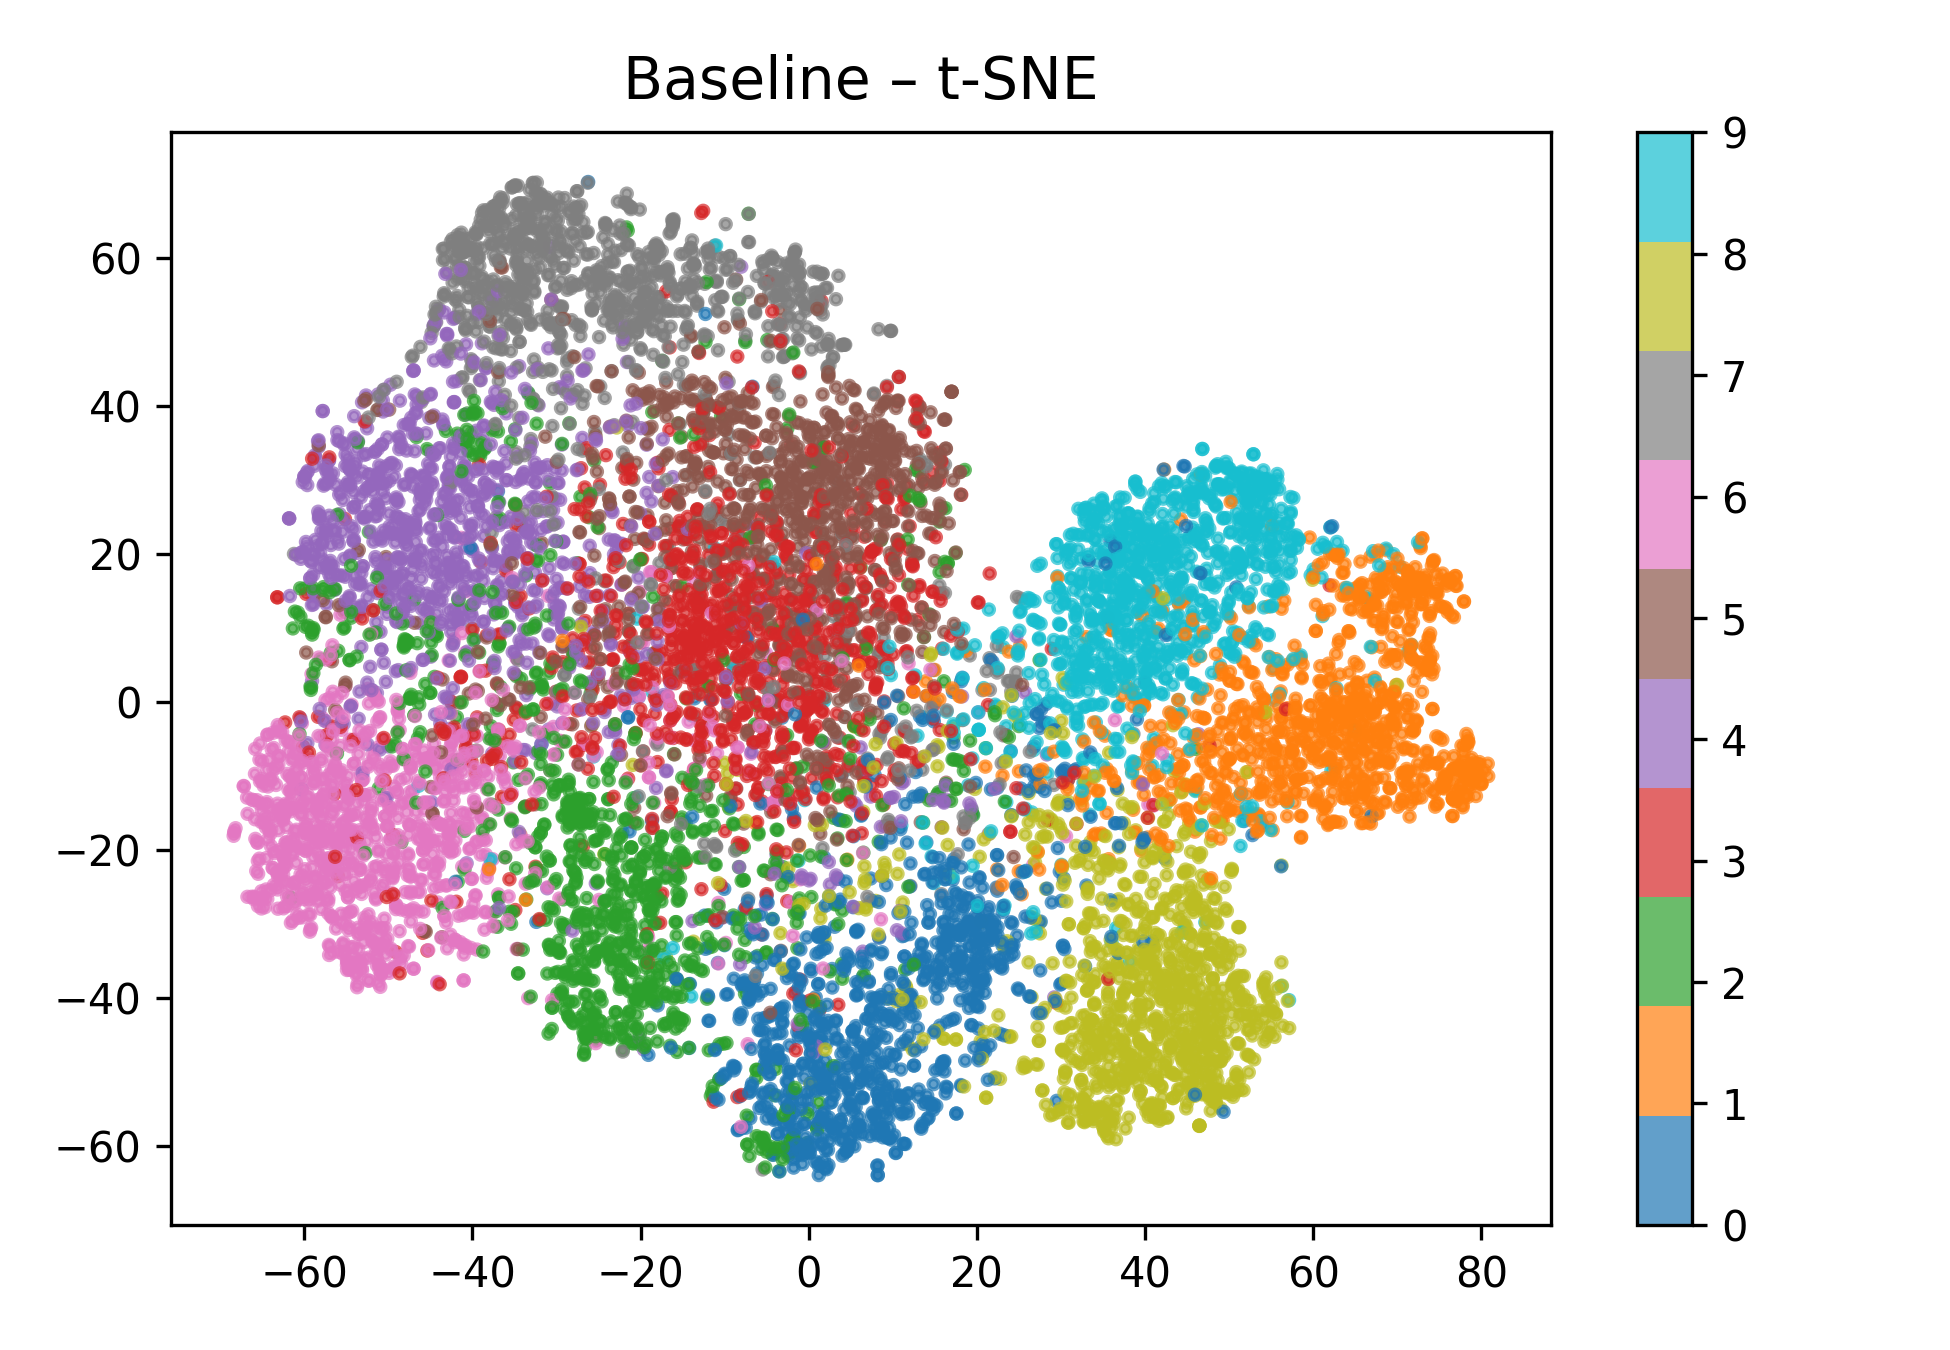
\includegraphics[width=0.45\textwidth]{figures/baseline_tsne.png}
\label{fig:chap4_tsne_baseline}
}
\subfigure[添加本章方法]{
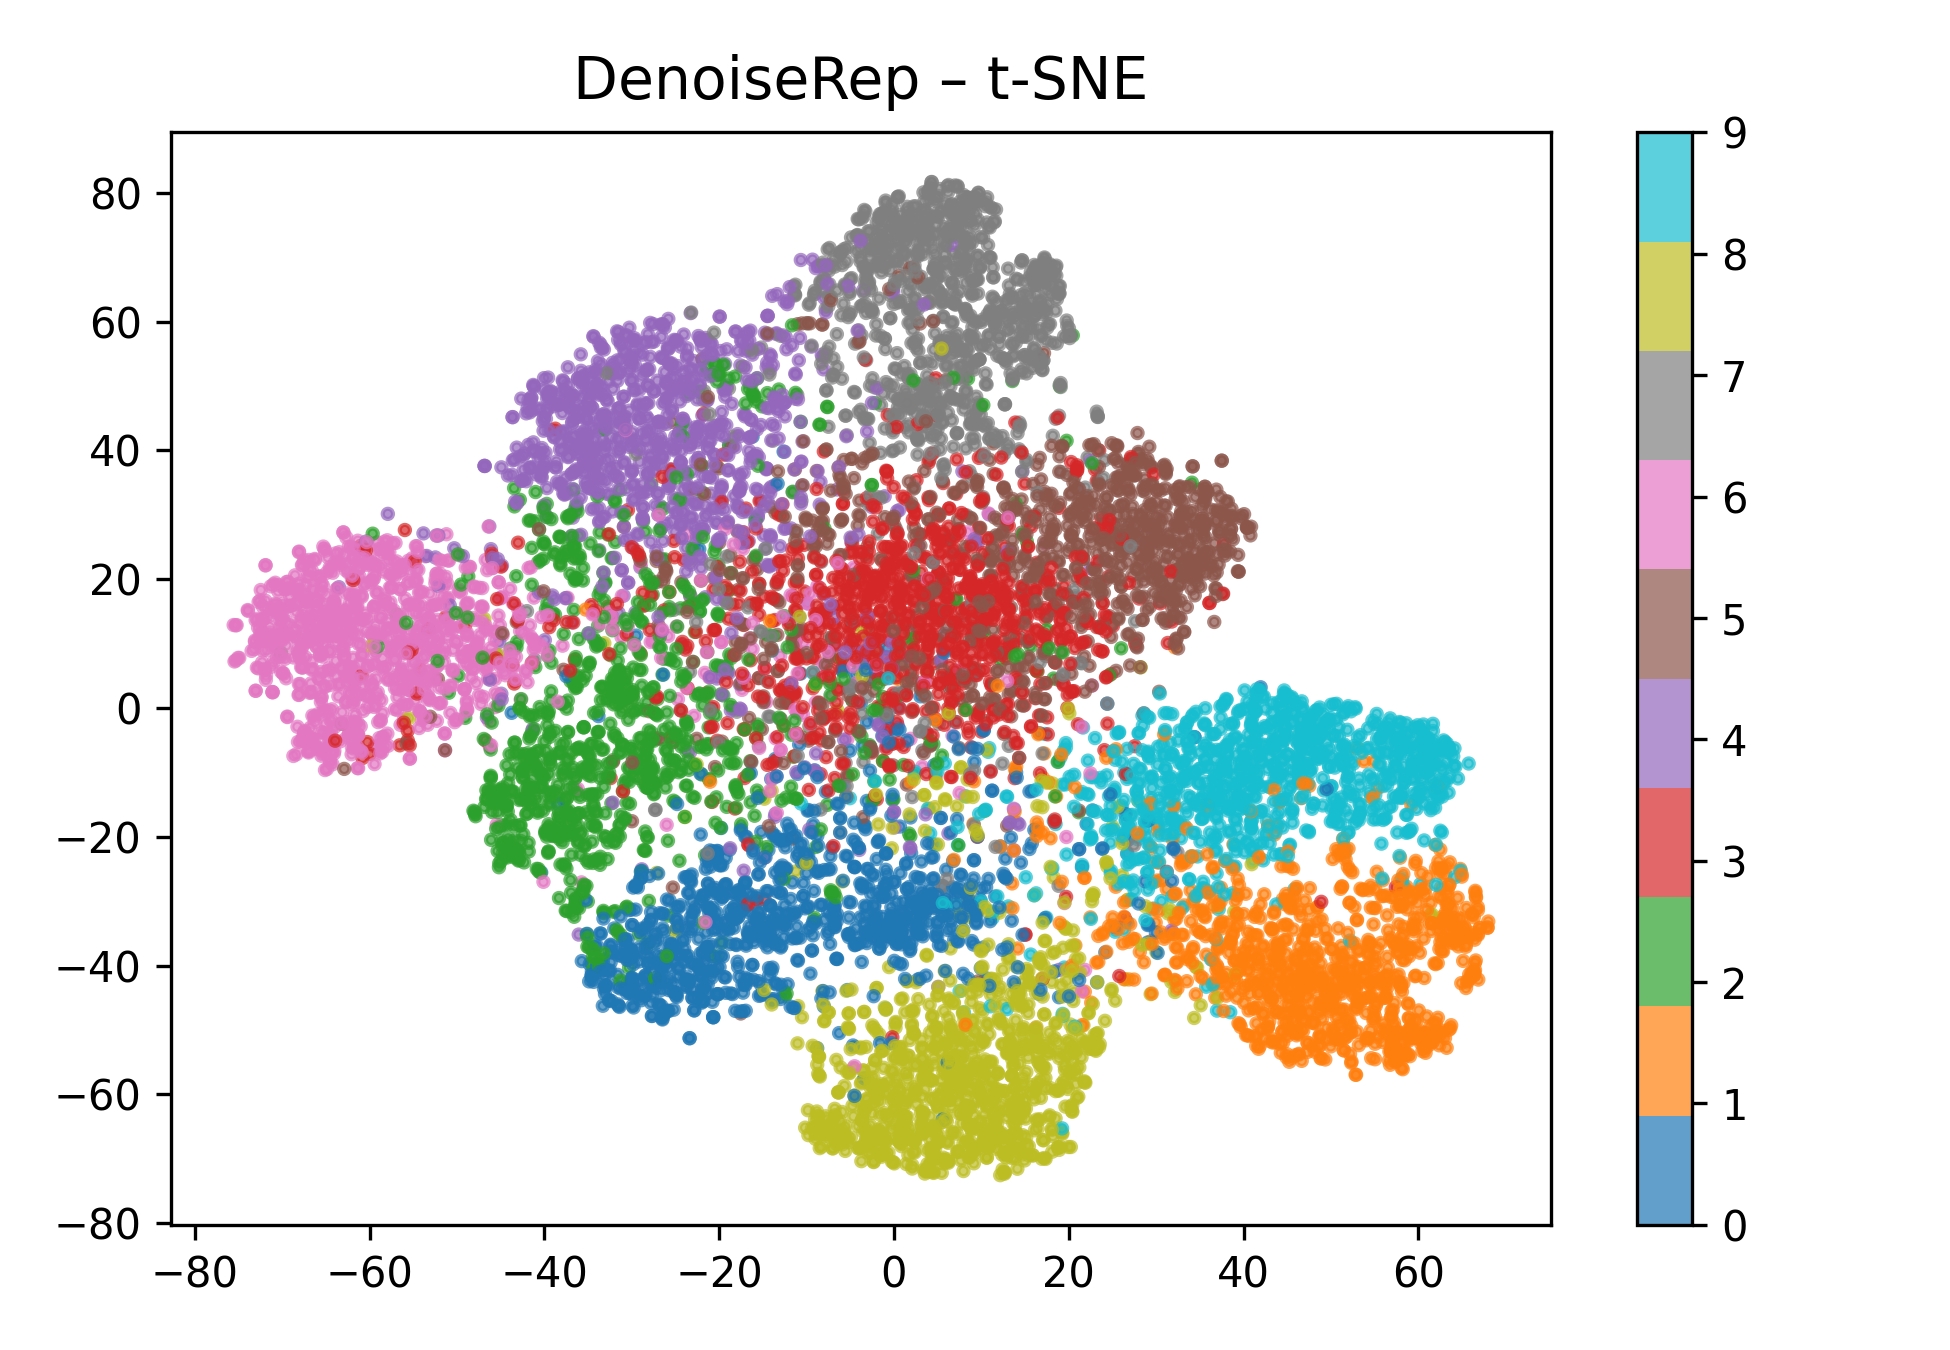
\includegraphics[width=0.45\textwidth]{figures/denoise_tsne.png}
\label{fig:chap4_tsne_denoise}
}
\caption{Cifar-10分类任务的t-SNE特征可视化对比\protect\\[-2pt]{\rm Fig.\;\thefigure\quad t-SNE visualization of features on Cifar-10 classification}}\label{fig:chap4_tsne}
\end{figure}

图\ref{fig:chap4_tsne}利用t-SNE\cite{maaten2008visualizing}将高维CLS特征降至二维空间进行可视化。可以观察到，基线模型（图\ref{fig:chap4_tsne_baseline}）的特征聚类存在明显的重叠区域，尤其是语义相近的类别（如"汽车"与"卡车"、"猫"与"狗"）在边界处存在严重混杂，反映了特征中残留噪声导致的类内分散和类间模糊。而添加本章方法后（图\ref{fig:chap4_tsne_denoise}），各类别的聚类变得更加紧凑，类间边界明显更加清晰，原本混杂的类别在特征空间中被有效分离。这一结果直观地表明，去噪增强能够降低特征中的噪声干扰，使同类样本的特征表示更加一致，不同类别之间的判别性更强。

\begin{figure}[htbp]
\centering
\subfigure[基线模型]{
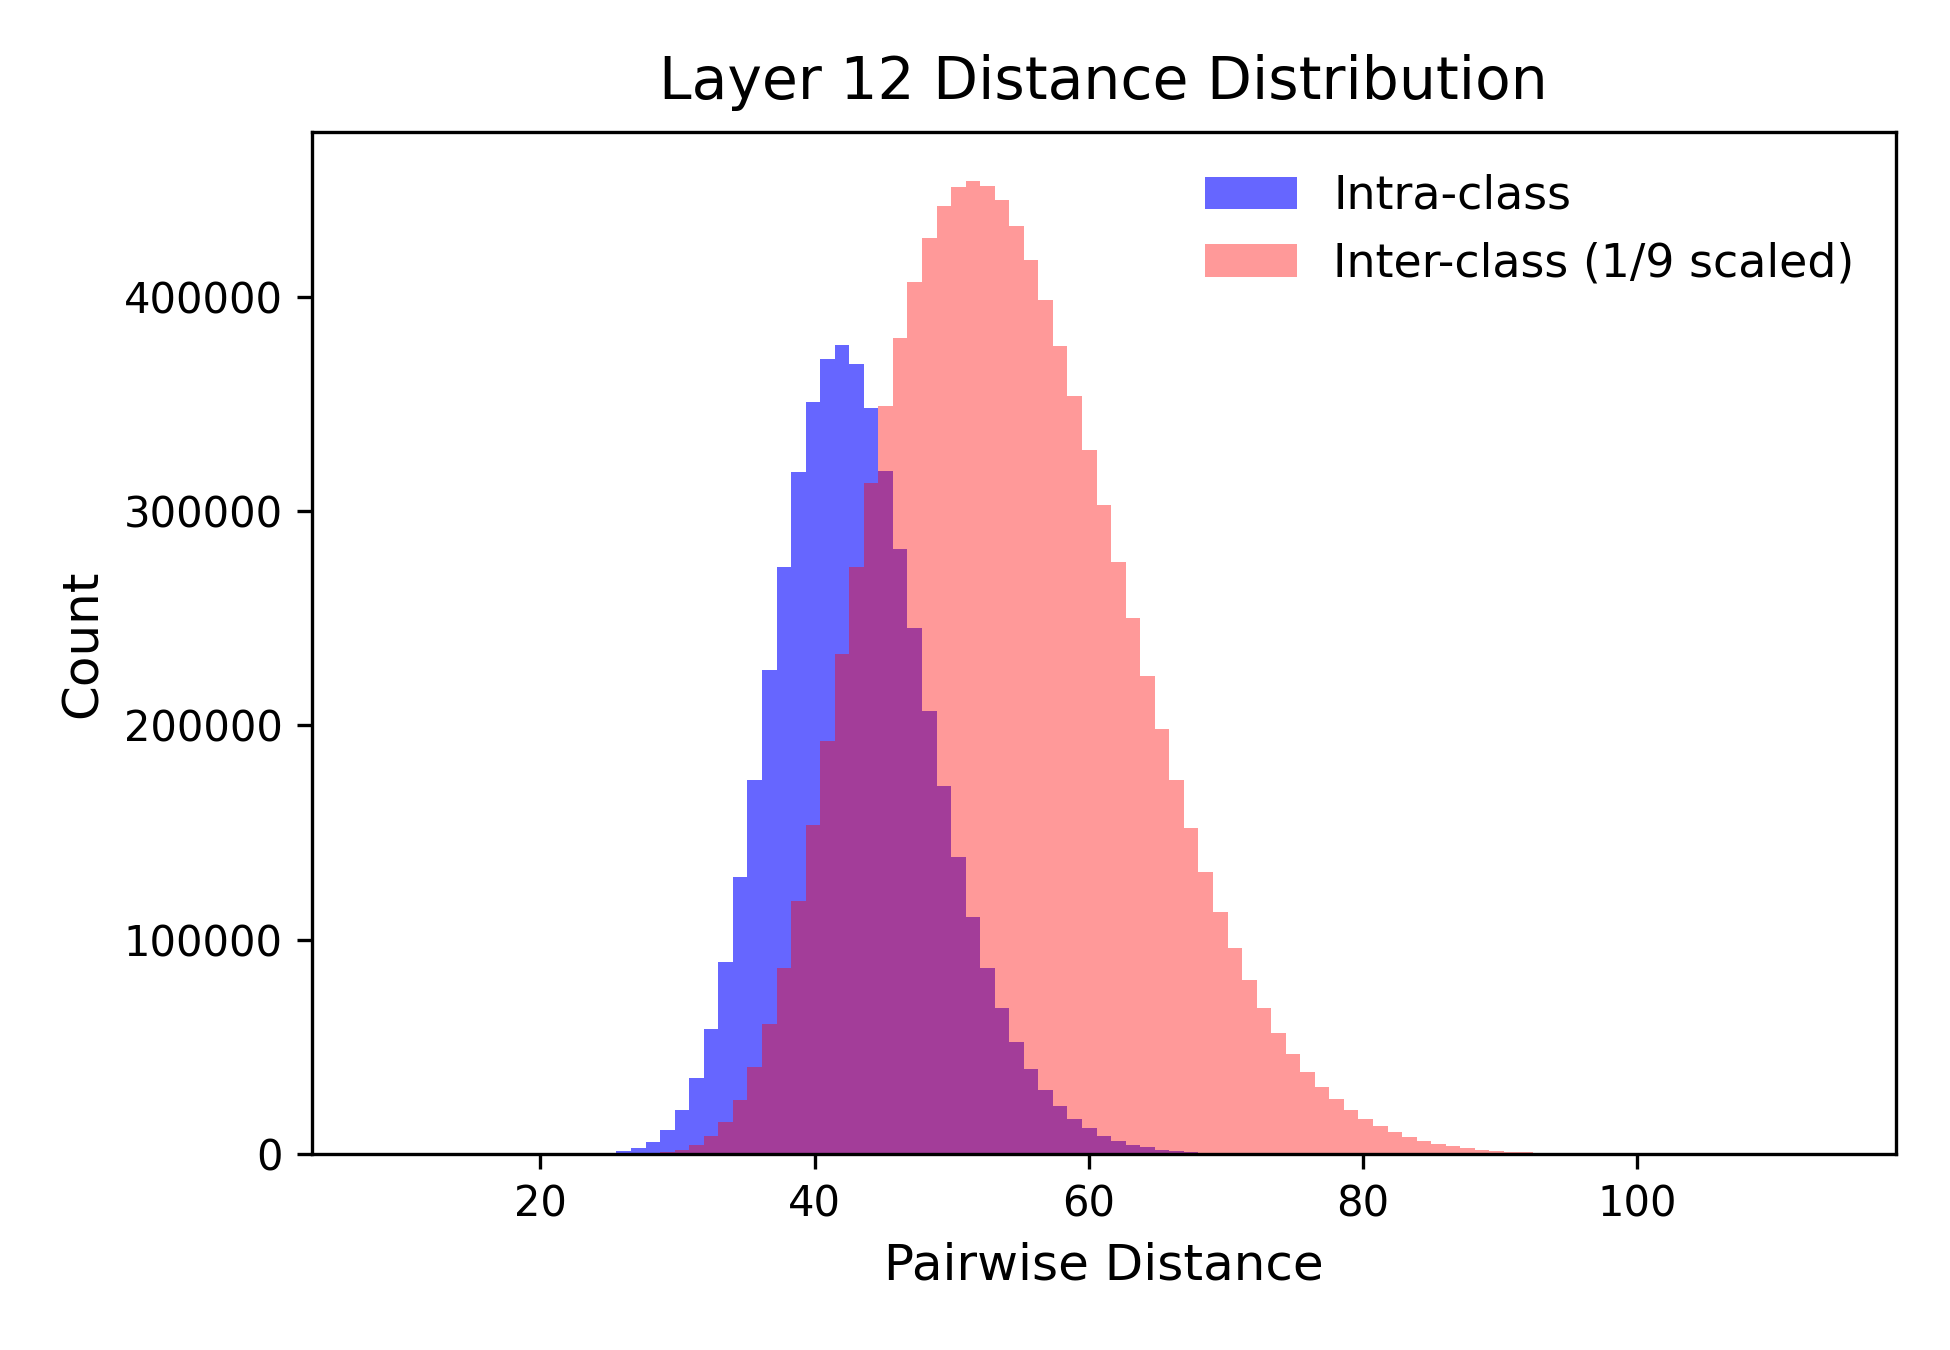
\includegraphics[width=0.45\textwidth]{figures/layer12_modelA.png}
\label{fig:chap4_dist_baseline}
}
\subfigure[添加本章方法]{
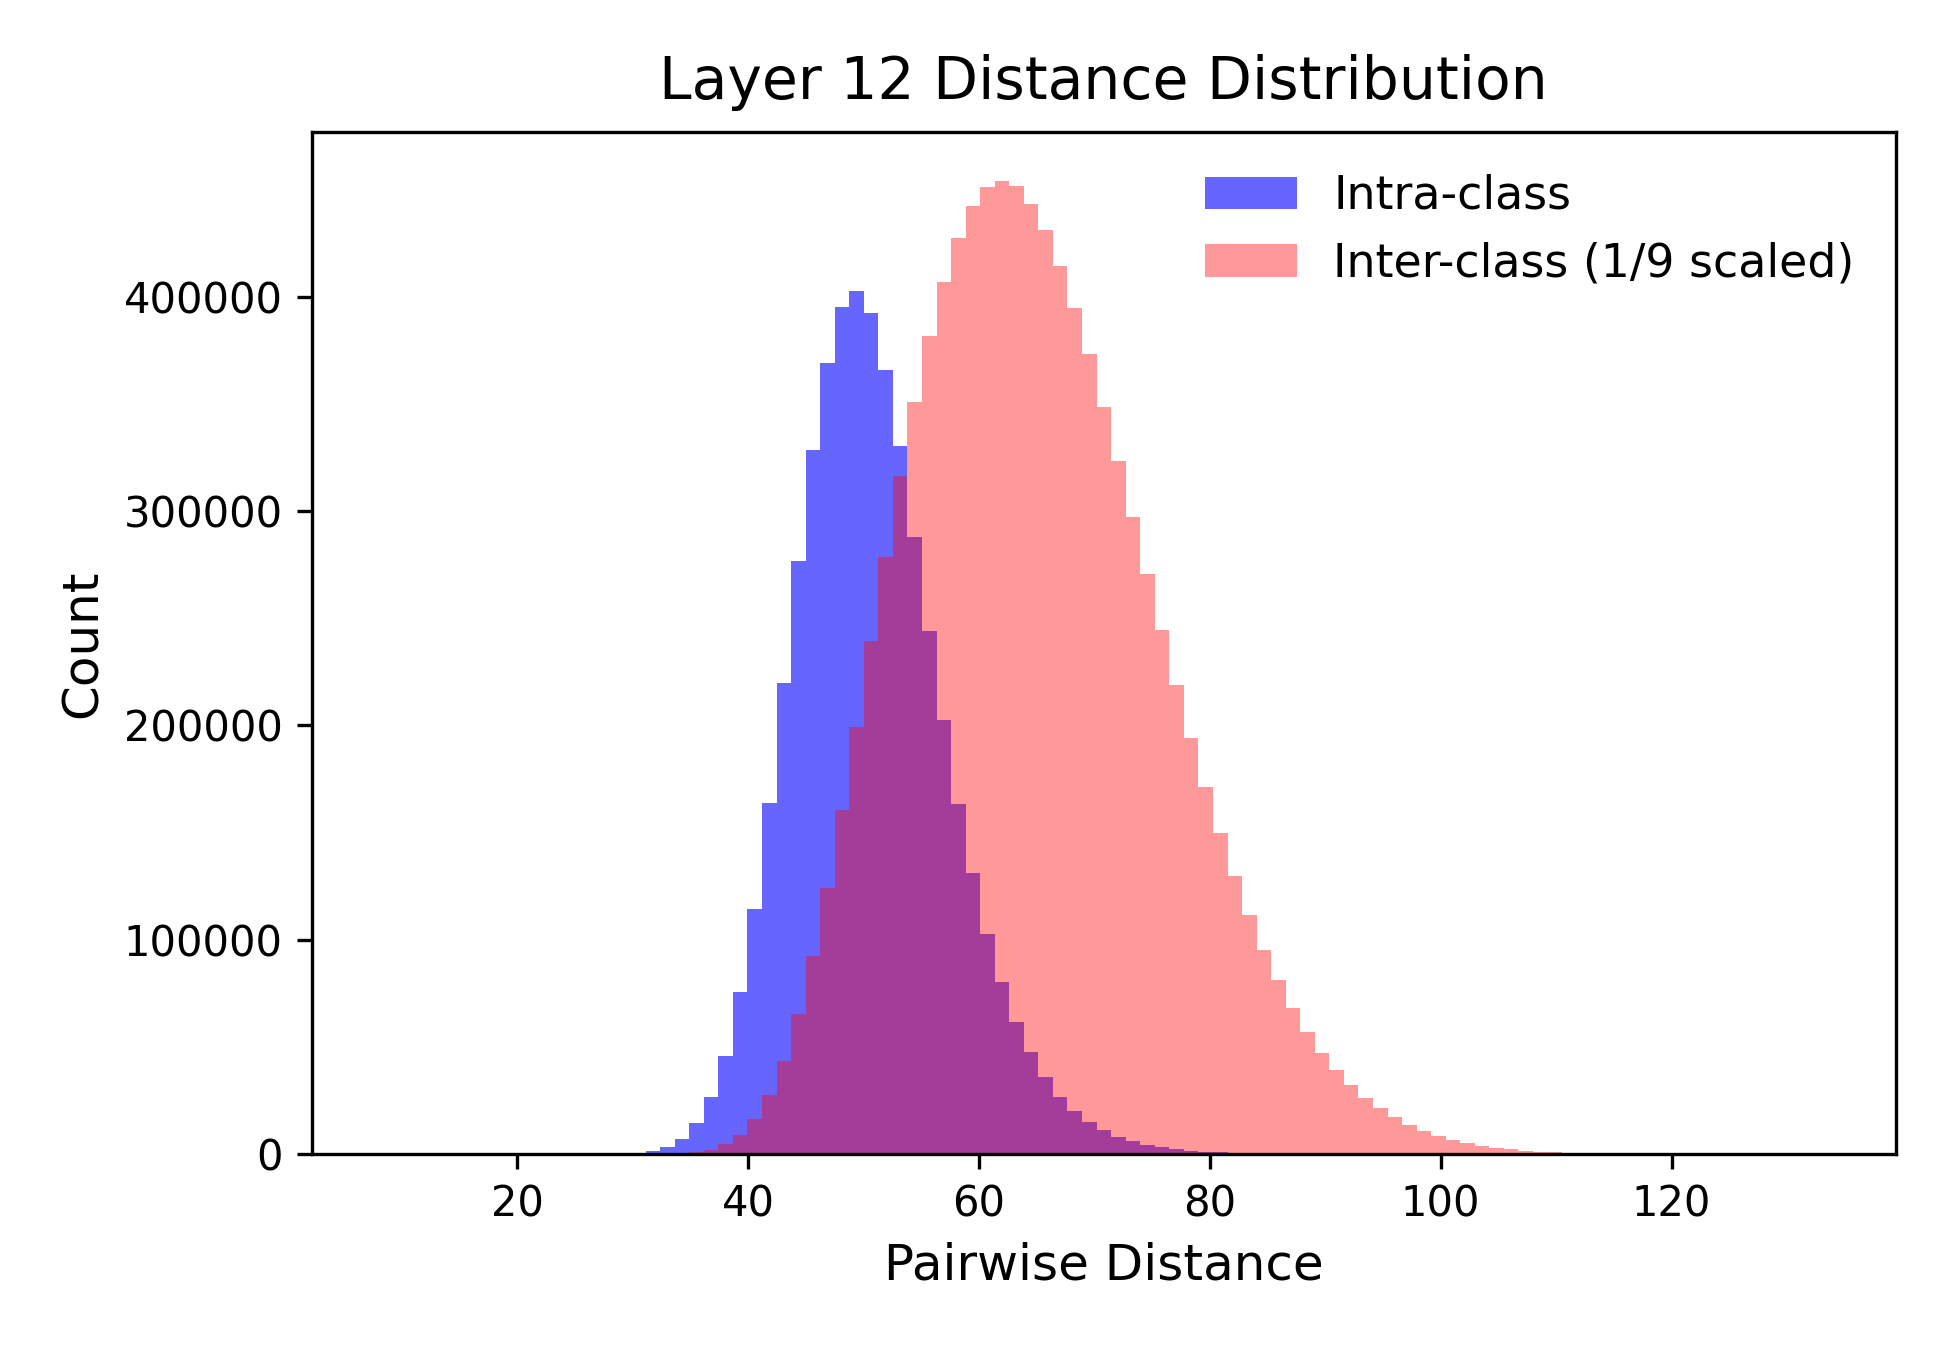
\includegraphics[width=0.45\textwidth]{figures/layer12_modelB.png}
\label{fig:chap4_dist_denoise}
}
\caption{类内距离与类间距离的直方图对比\protect\\[-2pt]{\rm Fig.\;\thefigure\quad Histogram comparison of intra-class and inter-class distances}}\label{fig:chap4_dist}
\end{figure}

为进一步定量验证上述观察，图\ref{fig:chap4_dist}展示了类内距离和类间距离分布的直方图对比。在基线模型中（图\ref{fig:chap4_dist_baseline}），类内距离和类间距离的分布存在较大的重叠区域，意味着部分不同类别的样本对之间的距离甚至小于同类样本对之间的距离，这将直接导致分类边界的模糊。添加本章方法后（图\ref{fig:chap4_dist_denoise}），类内距离分布向更小值集中（左移且变窄），类间距离分布向更大值偏移（右移），两个分布之间的重叠面积显著减少，表明去噪增强有效改善了特征空间的可分离性。

表\ref{tab:chap4_dist_stats}给出了定量统计结果（类内均值归一化为1）。

\begin{table}[htbp]
\centering
\caption{Cifar-10验证集上的类内/类间距离统计分析\protect\\[-2pt]{\rm Table\;\thetable\quad Statistical analysis of intra- and inter-class distances on Cifar-10}}\label{tab:chap4_dist_stats}
\vspace{0.2cm}
\renewcommand{\arraystretch}{1.2}
\begin{tabular}{l|c|c}
\hline\hline
指标 & 基线 & +本章方法 \\
\hline
类内方差 & 0.019 & 0.017 \\
类间均值 & 43.096 & 50.755 \\
类间方差 & 54.132 & 64.959 \\
类间/类内比 & 1.256 & 1.280 \\
重叠面积 & 0.463 & 0.416 \\
\hline\hline
\end{tabular}
\end{table}

统计结果与可视化分析一致：（1）类内方差从0.019降低至0.017（降幅10.5\%），说明同类样本的特征表示更加一致，去噪减少了类内特征的随机波动；（2）类间均值从43.096增加至50.755（增幅17.8\%），说明不同类别的特征中心在空间中被推得更远，判别性显著增强；（3）类间/类内比从1.256提高至1.280，说明特征空间的整体可分离性得到改善；（4）重叠面积从0.463降低至0.416（降幅10.2\%），说明类内和类间距离分布的分离程度更好，理论上的分类错误上界随之降低。这些结果从特征几何的角度充分证明了去噪增强对表征质量的改善。

\subsubsection{下游任务定性可视化}

为验证特征去噪在实际下游任务中的效果，本节分别对目标检测与实例分割、行人重识别两类任务进行定性可视化分析。

图\ref{fig:chap4_det_vis}展示了基线模型与添加本章方法后在COCO数据集上的目标检测与实例分割定性对比结果。

\begin{figure*}[htbp]
\centering
\subfigure[基线模型检测结果]{
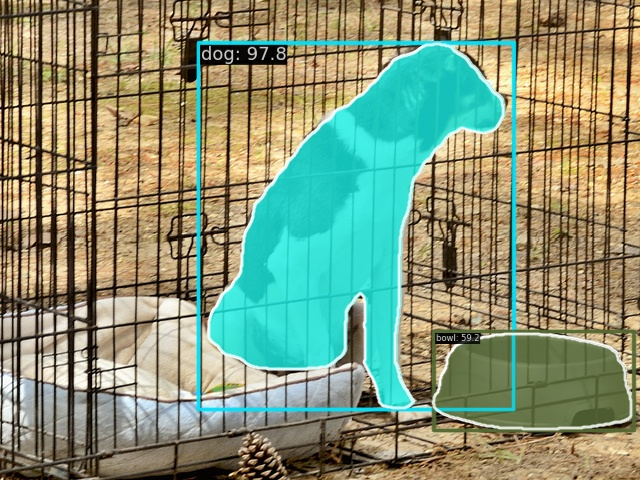
\includegraphics[width=0.19\textwidth]{figures/det_vis/base_01.jpg}\hfill
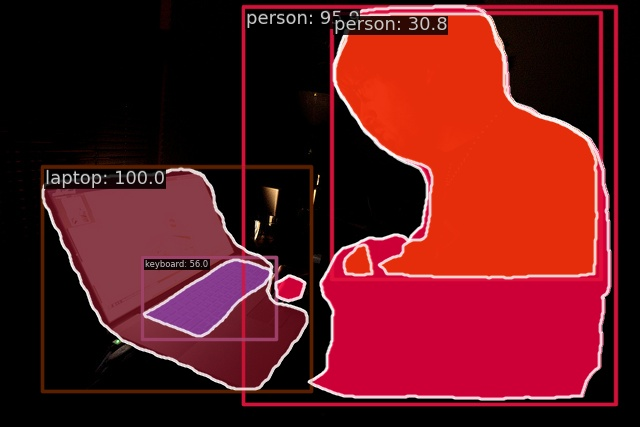
\includegraphics[width=0.19\textwidth]{figures/det_vis/base_03.jpg}\hfill
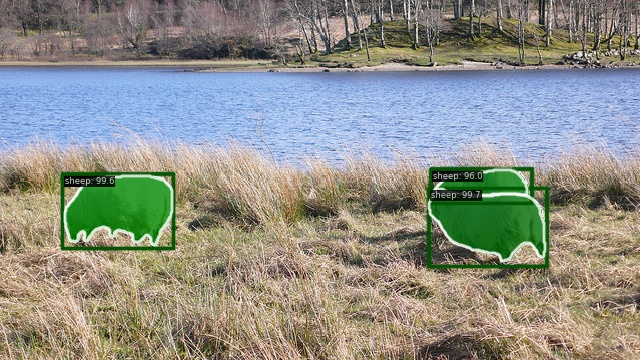
\includegraphics[width=0.19\textwidth]{figures/det_vis/base_04.jpg}\hfill
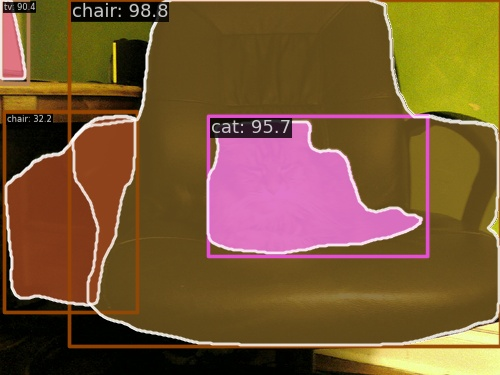
\includegraphics[width=0.19\textwidth]{figures/det_vis/base_05.jpg}\hfill
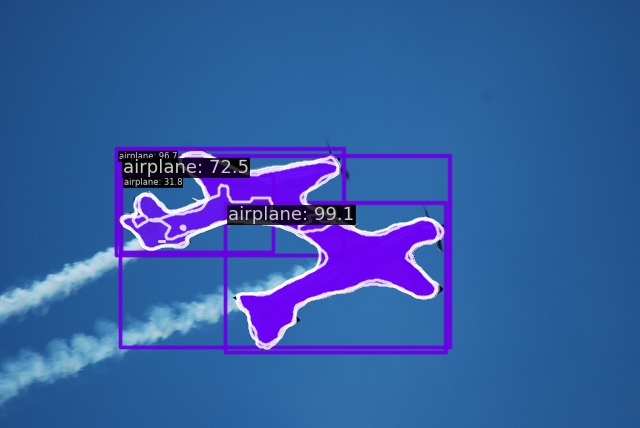
\includegraphics[width=0.19\textwidth]{figures/det_vis/base_06.jpg}
\label{fig:chap4_det_base}
}
\subfigure[添加本章方法后的检测结果]{
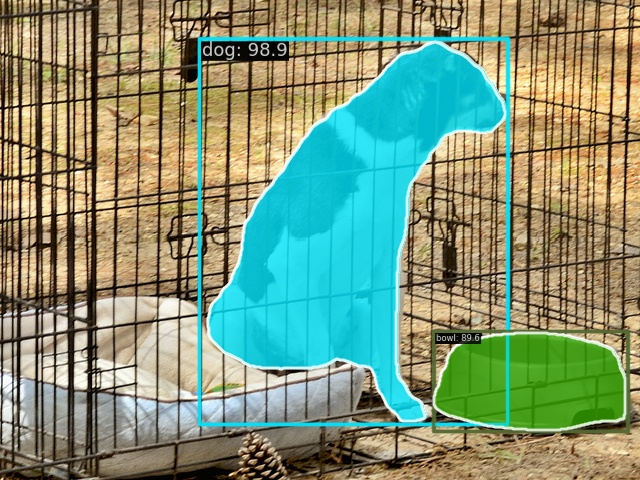
\includegraphics[width=0.19\textwidth]{figures/det_vis/denoiserep_01.jpg}\hfill
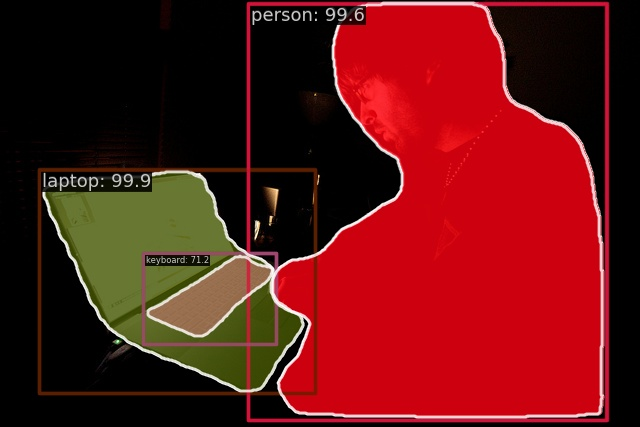
\includegraphics[width=0.19\textwidth]{figures/det_vis/denoiserep_03.jpg}\hfill
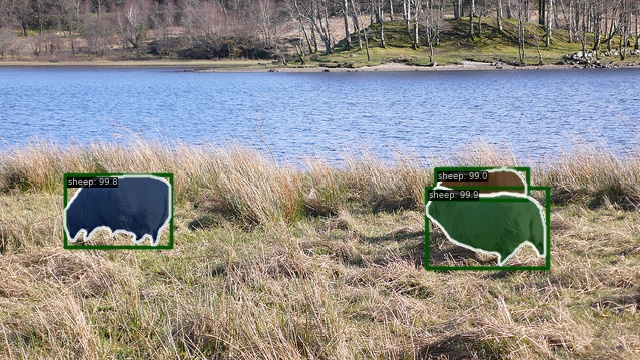
\includegraphics[width=0.19\textwidth]{figures/det_vis/denoiserep_04.jpg}\hfill
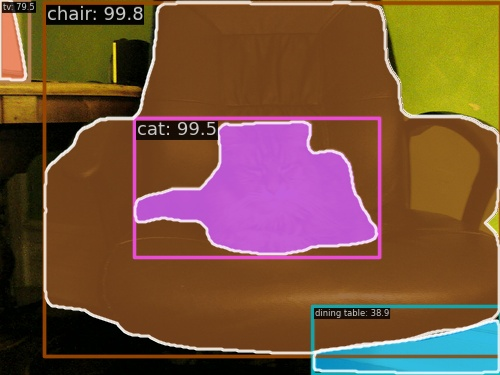
\includegraphics[width=0.19\textwidth]{figures/det_vis/denoiserep_05.jpg}\hfill
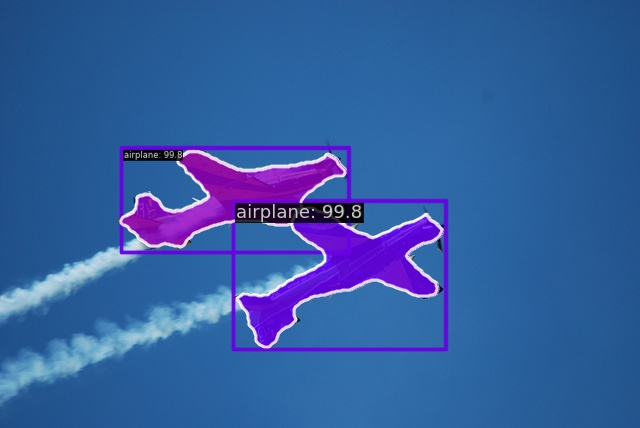
\includegraphics[width=0.19\textwidth]{figures/det_vis/denoiserep_06.jpg}
\label{fig:chap4_det_denoise}
}
\caption{目标检测与实例分割的定性对比\protect\\[-2pt]{\rm Fig.\;\thefigure\quad Qualitative comparison of object detection and instance segmentation results}}\label{fig:chap4_det_vis}
\end{figure*}

对比图\ref{fig:chap4_det_base}和图\ref{fig:chap4_det_denoise}，可以从以下几个维度观察去噪增强的效果：（1）在误检抑制方面，基线模型在背景杂乱的区域容易产生虚假检测响应，例如将背景纹理误识别为目标。添加本章方法后，这类误检被有效抑制，模型的精确率（Precision）得到改善。（2）在定位精度方面，去噪后的检测框与目标的贴合程度更高，边界框的回归更加精确，这与表\ref{tab:chap4_det}中AP$_{75}$（高IoU阈值下的AP）的提升相呼应。（3）在实例分割质量方面，去噪后的分割掩码边界更加光滑且贴合目标轮廓，尤其在目标边缘和遮挡区域表现更为明显。这些定性结果表明，特征去噪能够有效抑制噪声引起的虚假响应，提升密集预测任务中特征的空间精度和语义一致性。

图\ref{fig:chap4_reid_vis}展示了行人重识别任务中检索排序结果的定性对比。每行最左侧为查询（Query）图像，其后为按特征相似度从高到低排列的检索结果，绿色边框表示正确匹配（与查询为同一身份），红色边框表示错误匹配。

\begin{figure*}[htbp]
\centering
\subfigure[基线模型检索结果]{
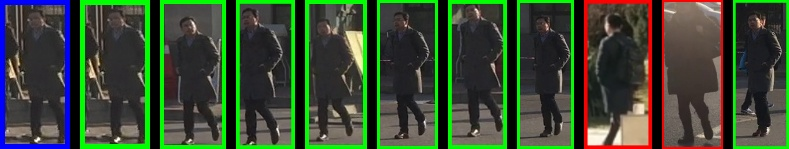
\includegraphics[width=0.95\textwidth]{figures/reid_vis/reid_base.jpg}
\label{fig:chap4_reid_base}
}
\subfigure[添加本章方法后的检索结果]{
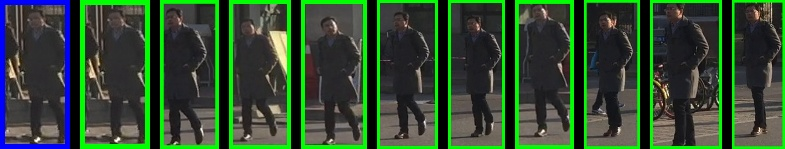
\includegraphics[width=0.95\textwidth]{figures/reid_vis/reid_denoise.jpg}
\label{fig:chap4_reid_denoise}
}
\caption{行人重识别检索排序结果的定性对比\protect\\[-2pt]{\rm Fig.\;\thefigure\quad Qualitative comparison of person re-identification ranking results}}\label{fig:chap4_reid_vis}
\end{figure*}

对比图\ref{fig:chap4_reid_base}和图\ref{fig:chap4_reid_denoise}可以发现，基线模型容易受到背景杂乱、相似服装颜色和光照变化等因素的干扰，在排序靠前的位置出现了多个错误匹配（红色边框）。这些错误匹配的共性特征是：与查询行人具有相似的背景环境或整体色调，但实际身份不同——说明基线模型的特征中混入了过多与身份无关的环境噪声。而添加本章方法后，模型提取的特征更加聚焦于身份判别性信息，错误匹配显著减少，排序前列几乎全部为正确匹配（绿色边框），检索排序的质量和可靠性大幅提升。

\subsubsection{注意力图可解释性分析}

前两节分别从特征分布和下游任务输出的角度验证了去噪增强的效果，但尚未揭示去噪如何影响模型的内部决策过程。为提供可解释性层面的理解，本节采用Attention Rollout\cite{abnar2020quantifying}方法对模型的注意力分布进行可视化分析。Attention Rollout通过递归地在所有Transformer层上聚合多头自注意力权重（取均值融合），将多层注意力传播关系压缩为一张整体注意力热力图，能够反映模型在推理时对输入图像各区域的关注程度。

图\ref{fig:chap4_attn_map}展示了DukeMTMC-reID数据集上四个代表性样本的注意力图对比。每个样本从左到右依次为：原始图像、基线注意力热力图、基线叠加图、本章方法注意力热力图、本章方法叠加图以及逐像素差异图（基线$-$本章方法）。

\begin{figure*}[htbp]
\centering
\subfigure[样本1：Pearson $r{=}0.827$，Att-IoU@0.5${=}0.521$]{
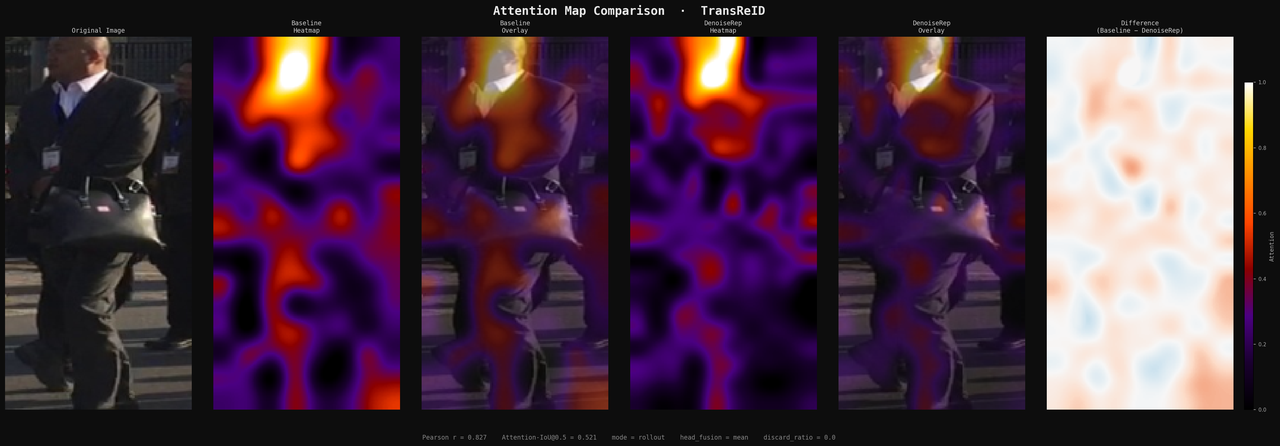
\includegraphics[width=0.48\textwidth]{figures/attn_reid_1.png}
\label{fig:chap4_attn1}
}\hfill
\subfigure[样本2：Pearson $r{=}0.811$，Att-IoU@0.5${=}0.537$]{
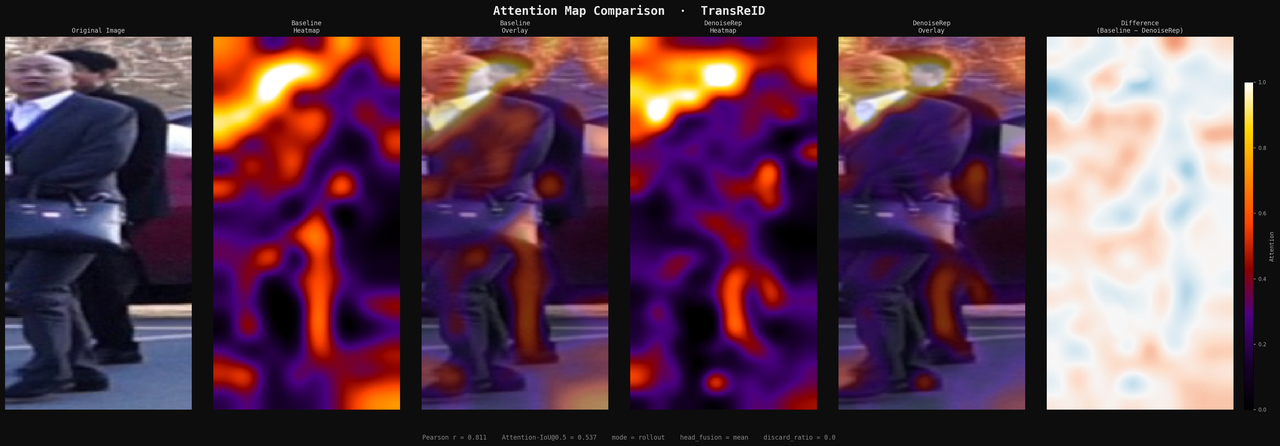
\includegraphics[width=0.48\textwidth]{figures/attn_reid_2.png}
\label{fig:chap4_attn2}
}
\subfigure[样本3：Pearson $r{=}0.641$，Att-IoU@0.5${=}0.489$]{
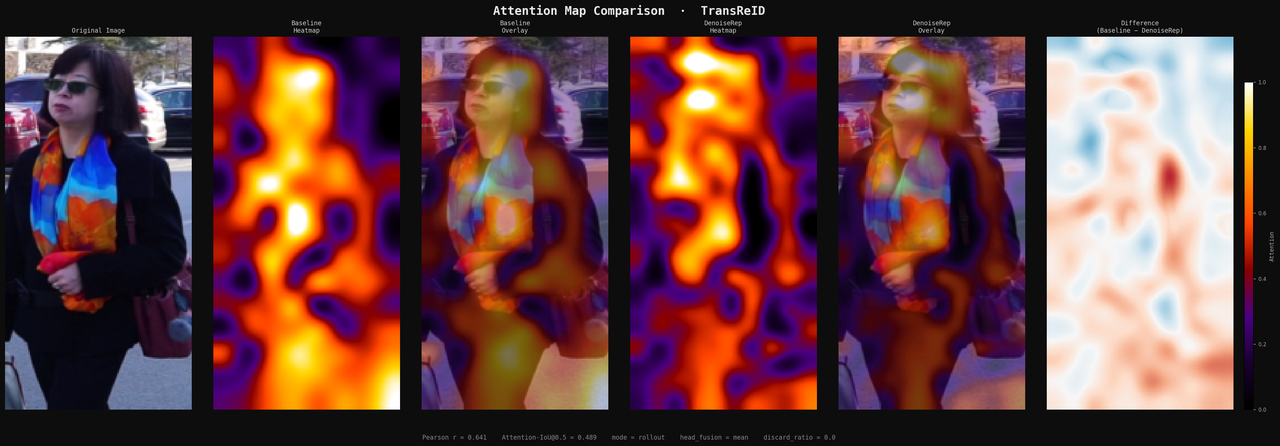
\includegraphics[width=0.48\textwidth]{figures/attn_reid_3.png}
\label{fig:chap4_attn3}
}\hfill
\subfigure[样本4]{
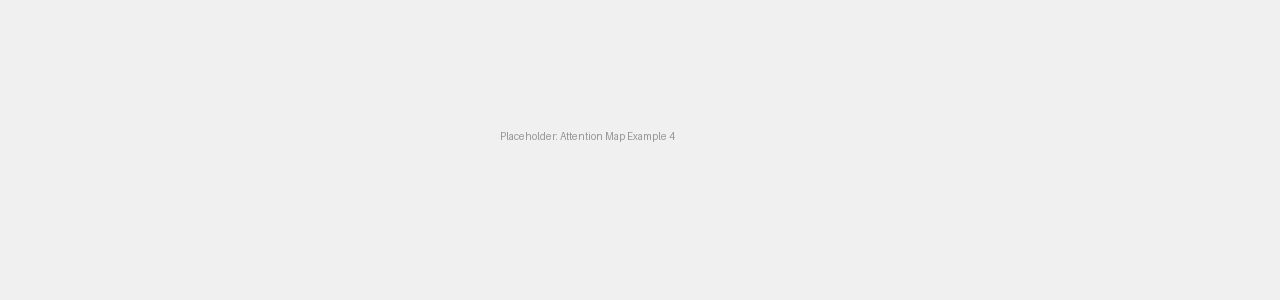
\includegraphics[width=0.48\textwidth]{figures/attn_reid_4.png}
\label{fig:chap4_attn4}
}
\caption{基线模型与本章方法在行人重识别任务上的注意力图对比（DukeMTMC-reID数据集）。去噪后模型的注意力更集中于具有身份判别性的区域，对背景干扰的响应显著降低\protect\\[-2pt]{\rm Fig.\;\thefigure\quad Attention map comparison between Baseline and our method on person re-identification (DukeMTMC-reID)}}\label{fig:chap4_attn_map}
\end{figure*}

从图\ref{fig:chap4_attn_map}中可以得出以下关键发现：

（1）去噪后的模型更加聚焦于具有身份判别性的区域。对比基线模型和本章方法的热力图，去噪后的模型将注意力更集中地分配在语义上有意义的身体区域——如面部、上半身和服装纹理等对身份判别至关重要的部位。以图\ref{fig:chap4_attn1}为例，基线模型的注意力在行人身体和背景行人之间分散分配，而去噪后的模型将注意力高度集中于目标行人的上半身和面部区域，有效过滤了背景中其他行人的干扰。

（2）环境噪声在去噪后受到的关注显著降低。差异图（最右列）清晰地展示了本章方法减少了对背景元素（如其他行人、街道设施和杂乱环境）的注意力分配。差异图中的暖色区域（正值差异）表示基线模型比去噪模型分配了更多注意力的区域，这些区域主要对应于背景干扰物。在图\ref{fig:chap4_attn3}中，这一现象尤为明显：基线模型对背景中的建筑物和路面分配了大量注意力，而去噪后这些区域的注意力权重被显著抑制。

（3）定量注意力指标证实了上述改善。为量化注意力聚焦程度的变化，本节计算了两个指标：注意力图与行人边界框掩码之间的Pearson相关系数$r$（衡量注意力与目标区域的整体相关程度）以及Attention-IoU@0.5（将注意力值阈值化后计算与真实行人区域的IoU，衡量注意力的空间聚焦精度）。结果显示Pearson $r$值范围为0.641至0.827，Att-IoU@0.5值范围为0.489至0.537，表明去噪后的注意力重新分配是精细化的身份感知聚焦，而非简单地将所有注意力集中到人体区域的空间定位，模型在保持对目标区域关注的同时，更加精准地区分了具有判别性的身体部位与非信息性的身体区域。

综合上述三个层次的可视化和可解释性分析，可以得出以下结论：特征级去噪通过抑制中间特征中的噪声成分，从根本上改变了模型的注意力分配模式——将注意力从任务无关的背景干扰物重新导向具有判别性的语义区域。这一机制不仅解释了本方法在检索和识别等任务上取得性能提升的内在原因，也为理解扩散模型去噪过程对判别式特征学习的影响提供了可解释性层面的依据。

\section{本章小结}
\label{sec:chap4_summary}

本章针对第三章方法存在的两个核心局限——轻量去噪模块的表达能力受限和单步去噪幅度有限，提出了基于模型蒸馏的特征增强算法。主要贡献和结论如下：

（1）提出了教师--学生蒸馏去噪框架。通过引入参数量不受约束的教师去噪网络在训练阶段指导学生去噪模块的学习，有效弥补了线性去噪模块容量不足导致的噪声预测偏差。蒸馏知识在训练完成后被固化到学生模块中，因此推理阶段无需教师网络，保持了零额外推理成本的特性。

（2）设计了多步去噪融合策略。从多轮单层去噪的数学推导出发，揭示了仿射去噪操作的递归叠加规律，进而设计了多步去噪融合训练方法。通过在教师网络中执行多步去噪并将其知识蒸馏到学生模块中，在不增加推理成本的条件下实现了更大幅度的去噪效果。

（3）建立了统一的无监督与有监督去噪增强框架。将第三章的参数融合方法和本章的蒸馏增强方法统一到同一训练框架中，使之既可作为无监督的正则化手段，也可利用标签信息引导有针对性的去噪。

（4）在图像分类、行人重识别、车辆重识别、目标检测、图像分割五类视觉判别任务以及序列推荐和自然语言表征学习两类跨领域任务上进行了系统实验。消融实验验证了蒸馏模块和融合模块各自的独立贡献及互补性；跨任务实验在14种骨干网络和8种下游方法上均取得了一致的性能提升；跨领域实验在推荐系统和自然语言处理任务上的成功进一步证明了方法的通用性——只要模型包含可表示为线性变换的嵌入层，本方法即可即插即用地提升表征质量。特征分布可视化、下游任务定性可视化和注意力图可解释性分析分别从特征几何、任务输出和模型决策三个层面，直观证明了去噪增强对表征质量的改善效果及其内在作用机理。